%##########################################################################
%                                                                     
%                         MuM LaTeX-Vorlage
%                                 
%            für Bachelor-, Projekt- und Masterarbeiten
%                       
%			 von
%            	Merlin Morlock (merlin.morlock@tuhh.de)
% 				Alexander Held (alexander.held@tuhh.de)
%                      
%                      
%
%##########################################################################


%##########################################################################
% Formatierungsoptionen

\documentclass[12pt,a4paper,twoside]{report}
% todonotes need to be disabled if tikz externalize is used
% \usepackage[disable]{luatodonotes}
\usepackage{luatodonotes}
\usepackage{shellesc}
%##########################################################################
%Bitte in Einstellungen.tex entsprechende Daten anpassen
%Bitte hier die Daten anpassen

\newcommand{\MScBSc}{2} % 0=Bachelorarbeit 1=Projektarbeit 2=Masterarbeit
\newcommand{\Sprache}{1} % 0=Deutsch 1=Englisch 
%Für Bachelor- und Projektarbeiten ist in der Regel Deutsch erwünscht. Bei Masterarbeiten unter Umständen auch Englisch. In jedem Fall gilt: Englische Ausarbeitungen nur nach Absprache mit Professor Seifried!!

% Wenn die Sprache geändert wird muss eventuell zweimal kompiliert werden um eine auftretende Fehlermeldung zu beheben.

\newcommand{\VornameDesStudenten}{Thies Lennart}
\newcommand{\NachnameDesStudenten}{Alff}
\newcommand{\Matrikelnummer}{21380139}
\newcommand{\Studiengang}{Student des Theoretischen Maschinenbaus} %bitte in diesem Stil lassen!
\newcommand{\Betreuer}{D.-A. Dücker, M.\,Sc.}

\newcommand{\NummerDerArbeit}{XXX} % {XXX} durch Nummer der Arbeit ersetzen --> bitte ca. 1 Woche vor Abgabe der Arbeit die Nummer beim Sekretariat am MuM erfragen

%Hier den Titel der Arbeit eintragen
\newcommand{\ThemaDerArbeit}{
	\Large
	\bf
	\hspace{20mm}An approach to\\
	\hspace{20mm}agile Maneuvering with\\
	\hspace{20mm}Hydrobatic Micro Underwater Robots\\
	\bf
	\vspace{10mm}}

\newcommand{\ThemaArbeitZweitSprache}{
	\normalsize
	\bf
	\hspace{20mm}Ein Ansatz für\\
	\hspace{20mm}agiles Manövrieren mit\\
	\hspace{20mm}kleinen hydrobatischen Unterwasserrobotern\\
	\bf}
%##########################################################################

\usepackage{lmodern}
\usepackage{changepage}
\usepackage{fontspec}
\usepackage{xkeyval}
\usepackage{subfig}
\usepackage{pgfplotstable}
\usepackage{shellesc}
\usepackage{longtable}
\usepackage{rotating}
\usepackage{ucs}
\usepackage{xspace}
\usepackage{ifthen}
% Standard Style-Files
\usepackage{amsmath,amssymb,amsthm}
% used for prescript
\usepackage{mathtools}
\ifthenelse{\equal{\Sprache}{0}}
	{\usepackage[ngerman]{babel}
	\usepackage[ngerman]{isodate}
	}{}
\ifthenelse{\equal{\Sprache}{1}}
	{\usepackage[ngerman,english]{babel}
	\usepackage[ngerman,english]{isodate}
	}{}
\usepackage{a4}
\usepackage{float} % If we use this package, we can force figures and tables to appear at a certain place. --> use \begin{figure}[H]
\usepackage{flafter} %prevent figures to be displayed before referencing
\usepackage{acro}
\usepackage{graphicx}
\usepackage{svg}
\usepackage{color}
\usepackage{bm}
\usepackage{import}
\usepackage{algorithm}
\usepackage[autostyle=true,german=quotes]{csquotes}
\usepackage[plainpages=false]{hyperref}
\usepackage{cleveref}
\hypersetup{%
	pdfborder = {0 0 0}
} %remove red boxes around section references
\usepackage{bookmark}
\usepackage{multirow}
\usepackage{tabularx}
% center X columns for tabularx
\renewcommand{\tabularxcolumn}[1]{>{\centering\arraybackslash} m{#1}}
\usepackage{booktabs}
\usepackage{fancyhdr}
% \usepackage{siunitx}
\usepackage{units}
\usepackage{calc} %to use \widthof to obtain length of content
\usepackage{esvect}

\usepackage{algpseudocode}

% tell TeX that it's infinitely bad to have widows and orphans
\widowpenalty10000
\clubpenalty10000

%%% TIKZ & PGFPLOTS
\usepackage{tikz}
\usepackage{pgfplots}


\usepackage{caption}
\captionsetup{format=hang} % ab zweiter Zeile wird Caption eingerückt



%prevent all capital letter header in table of contents:
\usepackage{etoolbox}
\patchcmd{\tableofcontents}{\MakeUppercase\contentsname}{\contentsname}{}{}
\patchcmd{\tableofcontents}{\MakeUppercase\contentsname}{\contentsname}{}{} %needs to be used twice to work!

% ############################################################################
% Inverse Suche mit xdvi und kile:
%
\usepackage{srcltx}
%

% Insitutseigene Style-Files
\usepackage{Styles/mum_styles}

% Seitenstil
\pagestyle{headings}

% Abstand zwischen Absaetzen
\setlength{\parskip}{1.5ex}

% Einrueckung der ersten Zeile eines Absatzes unterdruecken
\setlength{\parindent}{0pt}

% Grosszuegigere Wortabstaende
\sloppy

% Damit Bilder moeglichst da sind, wo man sie will
\setcounter{topnumber}{20}
\setcounter{bottomnumber}{20}
\setcounter{totalnumber}{20}
\renewcommand{\topfraction}{.9999}
\renewcommand{\bottomfraction}{.9999}
\renewcommand{\textfraction}{0}


%##########################################################################
% Sonderumgebungen
\newtheorem{definition}{Definition}[chapter]
% Aufruf mit \begin{definition}[zusatz]  text  \end{definition}
\newtheorem{satz}{Satz}[chapter]
% Aufruf mit \begin{satz}[zusatz]  text  \end{satz}

\theoremstyle{definition}
\newtheorem{beispiel}{Beispiel}[chapter]
% Aufruf mit \begin{beispiel}[zusatz]  text  \end{beispiel}
\newtheorem{algorithmus}{Algorithmus}[chapter]
% Aufruf mit \begin{algorithmus}[zusatz]  text  \end{algorithmus}
\floatstyle{ruled}
\newfloat{algorithm}{thp}{alg} 
\floatname{algorithm}{Algorithmus}

%##########################################################################
% Kopfzeilen definieren
\setlength{\headheight}{15pt}
\pagestyle{fancyplain}                               
% f"ur documentclass 'article':
%\renewcommand{\sectionmark}[1]{\markboth{#1}{}}
%\renewcommand{\subsectionmark}[1]{\markright{\thesubsection\ #1}}
% f"ur documentclass 'report':
\renewcommand{\chaptermark}[1]{\markboth{\thechapter \hspace{3mm}#1}{}}
\renewcommand{\sectionmark}[1]{\markright{\thesection\ #1}}
\cfoot[\fancyplain{}{}]{\fancyplain{}{}}
\lhead[\fancyplain{}{\small\bf\thepage}]%
{\fancyplain{}{\nouppercase{\small\bf\leftmark}}}
\rhead[\fancyplain{}{\small\bf\rightmark}]%
{\fancyplain{}{\nouppercase{\small\bf\thepage}}}
\renewcommand{\footrulewidth}{0pt}

%##########################################################################
% Abkürzungen definieren
% Tabelle
%\newcommand{\tabref}[1]{Tab.~\ref{#1}}
%
%\ifthenelse{\equal{\Sprache}{0}}
%	{% Abbildung
%	\newcommand{\figref}[1]{Abb.~\ref{#1}}
%	
%	% Gleichungs--Referenzen:
%	\renewcommand{\eqref}[1]{Gl.~(\ref{#1})}
%	}{}
%\ifthenelse{\equal{\Sprache}{1}}
%{% Abbildung
%	\newcommand{\figref}[1]{Fig.~\ref{#1}}
%	
%	% Gleichungs--Referenzen:
%	\renewcommand{\eqref}[1]{Eq.~(\ref{#1})}
%}{}

\addto\extrasngerman{\def\tableautorefname{Tab.}}
\addto\extrasngerman{\def\figureautorefname{Abb.}}
\addto\extrasngerman{\def\euqationautorefname{Gl.}}
\newcommand{\algorithmautorefname}{Algorithm}
\addto\extrasngerman{\def\algorithmautorefname{Alg.}}
\newcommand{\subfigureautorefname}{\figureautorefname}

%###########################################################################

\raggedbottom	%Sorgt beim Dokumenttyp book dafür, daß kein Ausgleich des unteren Seitenrandes durch Dehnung der Absatzabstände durchgeführt wird. \raggedbottom ist bei den Dokumenttypen article, report und letter bereits voreingestellt. ==> da es zu Problemen kam wird der Befehl hier nochmals explizit definiert

\usepackage{sectsty}								% Einstellen der Textformatierung der Überschriften
\allsectionsfont{\raggedright}						% Linksbündige Ausrichtung der Überschriften ==> sonst teilweise Blocksatz wobei Überschriften große unschöne weiße Lücken bekommen können

\graphicspath{{images/}}

 \DeclareAcronym{fcu}{short=FCU, long=\emph{flight control unit}}

\DeclareAcronym{ros}{short=ROS, long=\emph{Robot Operating System}}

\DeclareAcronym{tcpip}{short = TCP/IP, long = \emph{Transmission Control Protocol/Internet Protocol}}

\DeclareAcronym{esc}{short = ESC, long = \emph{electronic speed controller}}

\DeclareAcronym{uav}{short = UAV, long = \emph{unmanned aerial vehicle}}

\DeclareAcronym{imu}{short = IMU, long = \emph{inertial measurement unit}}

\DeclareAcronym{tdm}{short = TDM, long = \emph{time-division multiplexing}}

\DeclareAcronym{uart}{short = UART, long = \emph{universal asynchronous receiver transmitter}}

\DeclareAcronym{cobs}{short = COBS, long = \emph{consistent overhead byte stuffing}}

\DeclareAcronym{rssi}{short = RSSI, long = \emph{received signal strength indicator}}

\DeclareAcronym{uauv}{short = \mu AUV, long = \emph{micro autonomous underwater vehicle}}

\DeclareAcronym{auv}{short = AUV, long = \emph{autonomous underwater vehicle}}

\DeclareAcronym{rrt}{short = RRT, long = rapidly-exploring random tree}

\DeclareAcronym{fmm}{short = FMM, long = fast marching method}

% !TeX root = ../Thesis.tex
\pgfplotsset{compat=newest} %globally avoid intereference of ticks and yaxis labels in plots with tikz package

\usetikzlibrary{positioning, arrows, fit, backgrounds, chains, shapes, angles, quotes}
\usetikzlibrary{decorations.pathreplacing}
\usetikzlibrary{babel}
\usetikzlibrary{pgfplots.statistics}
\usepgfplotslibrary{polar}
\usepgfplotslibrary{groupplots}
\usepgfplotslibrary{external}
\usetikzlibrary{pgfplots.groupplots}
\usetikzlibrary{patterns} %for patterns in bar plot
\pgfplotsset{plot coordinates/math parser=false}

%% e.g. pdflatex -synctex=1 -interaction=nonstopmode -shell-escape %.tex  is needed for using tikzexternalize!
\usetikzlibrary{external} %save tikz pictures as pdf and if not changed just use the pdf==>much faster compilation
% \tikzexternalize	% ACHTUNG: falls \usepackage{pdfpages} genutzt werden soll muss dieses zuerst deklariert werden und DANACH erst \tikzexternalize[optimize command away=\includepdf], mit diesem 						“away” Zusatz.

\makeatletter				% use this to define TiKZ paths for images AND ADD THE BELOW BEFORE INPUTTING EACH CHAPTER
\newcommand{\useexternalfile}[1]{%
	\tikzsetnextfilename{#1-output}%
	\input{\tikzexternal@filenameprefix#1.tikz}}
\makeatother
%%

\makeatletter
\pgfplotsset{
    boxplot/hide outliers/.code={
        \def\pgfplotsplothandlerboxplot@outlier{}%
    }
}
\makeatother


\pgfplotsset{every axis/.append style={cycle list={
			{mumblue},
			{mumred},
			{mumgreen},
			{mumorange},
			{mumteal}
}}}


\tikzsetexternalprefix{Bilder/externalize/}

\tikzset{%
	>=triangle 45,
	proto base/.style={
		rectangle, draw, minimum height=0.8cm, align=center, text width=1.0cm, thick
	},
	proto block/.style n args={1}{
		append after command={
			\pgfextra{
				\node[below=of \tikzlastnode, yshift=-0.2cm] {\normalsize #1};
			}
		}
	},
	proto header/.style={fill=green!30},
	proto marker/.style={fill=red!30},
	proto data/.style={fill=gray!30},
	proto block/.default={0}{-2cm},
	proto short/.style n args={1}{
		proto base,
		proto block={#1}
	},
	proto long/.style n args={1}{proto block={#1}, proto base, text width=2cm},
	proto vlong/.style n args={1}{proto block={#1}, proto base, text width=},
	show curve controls/.style={
		postaction={
			decoration={
				show path construction,
				curveto code={
					\draw [blue] 
					(\tikzinputsegmentfirst) -- (\tikzinputsegmentsupporta)
					(\tikzinputsegmentlast) -- (\tikzinputsegmentsupportb);
					\fill [red, opacity=0.5] 
					(\tikzinputsegmentsupporta) circle [radius=.5ex]
					(\tikzinputsegmentsupportb) circle [radius=.5ex];
				}
			},
			decorate
	}}
}

\pgfplotsset{
	every axis/.append style={legend cell align={left}, font=\footnotesize, axis line style=thick, ylabel near ticks, xlabel near ticks},
	every major tick/.append style={black, thick},
	/pgf/number format/use comma
}

\newcommand{\ubar}[1]{\underaccent{\bar}{#1}}

\newcommand{\Mrigid}{\Mb_\text{RB}}
\newcommand{\Madded}{\Mb_\text{A}}
\newcommand{\Mvadded}{\Mb_{v, \text{A}}}
\newcommand{\Crigid}{\Cb_\text{RB}}
\newcommand{\Cadded}{\Cb_\text{A}}
\newcommand{\Dadded}{\Db_\text{A}}
\newcommand{\Dvadded}{\Db_{v,\text{A}}}
\newcommand{\Domegaadded}{\Db_{\omega,\text{A}}}
\newcommand{\Jadded}{\Jb_\text{A}}

\newcommand{\vlinbody}{\prescript{\mathcal{B}}{}{\vb}}
\newcommand{\vlinbodydot}{\prescript{\mathcal{B}}{}{\vbp}}
\newcommand{\vangbody}{\prescript{\mathcal{B}}{}{\omeb}}
\newcommand{\vangbodyx}{\prescript{\mathcal{B}}{}{\omeb_x}}
\newcommand{\vangbodyy}{\prescript{\mathcal{B}}{}{\omeb_y}}
\newcommand{\vangbodyz}{\prescript{\mathcal{B}}{}{\omeb_z}}
\newcommand{\vangbodydot}{\prescript{\mathcal{B}}{}{\omebp}}
\newcommand{\aangbody}{\prescript{\mathcal{B}}{}{\omebp}}
\newcommand{\pworld}{\prescript{\mathcal{W}}{}{\pbo}}
\newcommand{\pworlddot}{\prescript{\mathcal{W}}{}{\pbp}}
\newcommand{\pworldddot}{\prescript{\mathcal{W}}{}{\pbpp}}
\newcommand{\vlinworld}{\prescript{\mathcal{W}}{}{\pbp}}
\newcommand{\vangworld}{\Thebp_{\mathcal{W}\mathcal{B}}}
\newcommand{\Rbodyworld}{\prescript{\mathcal{W}}{}{\Rb_\mathcal{B}}}
\newcommand{\TbodyWorld}{\Tb_\Theta}

\newcommand{\inputbody}{\prescript{\mathcal{B}}{}{\ub}}

\newcommand{\exbodyinworld}{\prescript{\mathcal{W}}{}{\eb}_{x\mathcal{B}}}
\newcommand{\eybodyinworld}{\prescript{\mathcal{W}}{}{\eb}_{y\mathcal{B}}}
\newcommand{\ezbodyinworld}{\prescript{\mathcal{W}}{}{\eb}_{z\mathcal{B}}}

\newcommand{\exdesiredbodyinworld}{\prescript{\mathcal{W}}{}{\eb}_{x\mathcal{B},\text{des}}}
\newcommand{\eydesiredbodyinworld}{\prescript{\mathcal{W}}{}{\eb}_{y\mathcal{B},\text{des}}}
\newcommand{\ezdesiredbodyinworld}{\prescript{\mathcal{W}}{}{\eb}_{z\mathcal{B},\text{des}}}

\newcommand{\exbody}{\eb_{x\mathcal{B}}}
\newcommand{\eybody}{\eb_{y\mathcal{B}}}
\newcommand{\ezbody}{\eb_{z\mathcal{B}}}

\newcommand{\bodyframeorigin}{O_{\mathcal{B}}}

\newcommand{\inputesci}{u_{\text{ESC},i}}
\newcommand{\ForceLinCoeffi}{\kappa_{f_{\text{lin}}, i}}
\newcommand{\ForceQuadCoeffi}{\kappa_{f_{\text{quad}}, i}}
\newcommand{\MomentLinCoeffi}{\kappa_{m_{\text{lin}}, i}}
\newcommand{\MomentQuadCoeffi}{\kappa_{m_{\text{quad}}, i}}


\newcommand{\vehiclestate}{\bm{\sigma}}
\newcommand{\pbppp}{\mbox{$\dddot{\bm{p}}$}\xspace}
\newcommand{\pppp}{\mbox{$\dddot{p}$}\xspace}

\newcommand{\fmax}{\mbox{$f_\text{max}$}\xspace}
\newcommand{\fmin}{\mbox{$f_\text{min}$}\xspace}
\newcommand{\omegamax}{\mbox{$\omega_\text{max}$}\xspace}
\newcommand{\omegamaxsquare}{\mbox{$\omega_\text{max}^2$}\xspace}
\newcommand{\fmaxsquare}{\mbox{$f_\text{max}^2$}\xspace}
\newcommand{\fminsquare}{\mbox{$f_\text{min}^2$}\xspace}

\newcommand{\fmaxaxis}{\mbox{$\bar{f}_k$}\xspace}
\newcommand{\fminaxis}{\mbox{$\ubar{f}_k$}\xspace}

\newcommand{\ximaxaxis}{\mbox{$\bar{\xi}_k$}\xspace}
\newcommand{\ximinaxis}{\mbox{$\ubar{\xi}_k$}\xspace}

\newcommand{\vangdesiredworld}{\prescript{\mathcal{W}}{}{\omeb_{\text{des}}}}\newcommand{\vangdesiredbody}{\prescript{\mathcal{B}}{}{\omeb_{\text{des}}}}
\newcommand{\vangerror}{\eb_{\omega}}
\newcommand{\aangerror}{\eb_{\dot{\omega}}}
\newcommand{\aangdesiredbody}{\prescript{\mathcal{B}}{}{\omebp_{\text{des}}}}
\newcommand{\thrustdesiredworld}{\prescript{\mathcal{W}}{}{\fb_{\text{des}}}}

\newcommand{\qdesired}{\qb_{\text{des}}}
\newcommand{\qactual}{\qb}
\newcommand{\qerror}{\qb_{\text{e}}}
\newcommand{\qerrorPY}{\qb_{\text{e,\theta\psi}}}


\newcommand{\KpBodyRate}{\Kb_{\text{P},\omega}}
\newcommand{\KiBodyRate}{\Kb_{\text{I},\omega}}
\newcommand{\KdBodyRate}{\Kb_{\text{D},\omega}}


\newcommand{\scr}[1]{\scriptsize{#1}}
\newcommand{\fs}[1]{\footnotesize{#1}} % required for pdf_tex
\newcommand{\ffs}[1]{\scriptsize{#1}}  % required for pdf_tex


\DeclareMathOperator{\absolute}{abs}

\newlength\shlength
\newcommand\xshlongvec[2][0]{\setlength\shlength{#1pt}%
	\stackengine{-5.6pt}{$#2$}{\smash{$\kern\shlength%
			\stackengine{7.55pt}{$\mathchar"017E$}%
			{\rule{\widthof{$#2$}}{.57pt}\kern.4pt}{O}{r}{F}{F}{L}\kern-\shlength$}}%
	{O}{c}{F}{T}{S}}


\begin{document}

%###########################################################################
%
%   Titelseite
%
%###########################################################################
\begin{titlepage}

\hspace{20mm}\begin{minipage}{0.3\linewidth}
		 \ifthenelse{\equal{\MScBSc}{0}}
			{\ifthenelse{\equal{\Sprache}{0}}
				{\textbf{Bachelorarbeit}\\
				\large{BSC-\NummerDerArbeit}}{}
			\ifthenelse{\equal{\Sprache}{1}}
			{\textbf{Bachelor's Thesis}\\
				\large{BSC-\NummerDerArbeit}}{}
			}{}
		\ifthenelse{\equal{\MScBSc}{1}}
			{\ifthenelse{\equal{\Sprache}{0}}
				{\textbf{Projektarbeit}\\
				\large{PRO-\NummerDerArbeit}}{}
				\ifthenelse{\equal{\Sprache}{1}}
				{\textbf{Project Thesis}\\
				\large{PRO-\NummerDerArbeit}}{}
			}{}
		\ifthenelse{\equal{\MScBSc}{2}}
			{\ifthenelse{\equal{\Sprache}{0}}
				{\textbf{Masterarbeit}\\
				\large{MSC-\NummerDerArbeit}}{}
				\ifthenelse{\equal{\Sprache}{1}}
				{\textbf{Master's Thesis}\\
				\large{MSC-\NummerDerArbeit}}{}
			}{}

	 	 
\end{minipage}\hfill
\begin{minipage}{0.3\linewidth}
	
\includegraphics[height=45pt]{Styles/mum_logo.pdf}
\end{minipage}
\vspace{8mm}
\begin{center}
	\vspace{10mm}
    {\ThemaDerArbeit}
	%\vspace{2mm}
	{\ThemaArbeitZweitSprache}
	\vspace{10mm}
	\ifthenelse{\equal{\Sprache}{0}}
	{\hspace{20mm}{\normalsize von}\large\\
	}{}
	\ifthenelse{\equal{\Sprache}{1}}
	{\hspace{20mm}{\normalsize by}\large\\
	}{}
	\hspace{20mm}{\large \VornameDesStudenten \ \NachnameDesStudenten}\\
	\vspace{15mm}
	\normalsize
	\ifthenelse{\equal{\Sprache}{0}}
	{	\hspace{20mm}\begin{tabular}{rl}
			Betreuer: & Prof. Dr.-Ing. R. Seifried \\
			& \Betreuer
		\end{tabular}\\
			\vfill
			\large
			\hspace{20mm}Technische Universität Hamburg (TUHH) \\
			\hspace{20mm}Institut für Mechanik und Meerestechnik\\
			\hspace{20mm}Prof.\ Dr.-Ing.\ R.\ Seifried
		}{}
	\ifthenelse{\equal{\Sprache}{1}}
	{	\hspace{20mm}\begin{tabular}{rl}
			Supervisors: & Prof. Dr.-Ing. R. Seifried \\
			& Prof. Dr.-Ing. B.-C. Renner \\
			& \Betreuer
		\end{tabular}\\
			\vfill
			\large
			\hspace{20mm}Hamburg University of Technology (TUHH) \\
			\hspace{20mm}Institute of Mechanics and Ocean Engineering\\
			\hspace{20mm}Prof.\ Dr.-Ing.\ R.\ Seifried
		}{}

\end{center}
\vspace{0.5cm}
\begin{center}
	\ifthenelse{\equal{\Sprache}{0}}
	{		{\large \hspace{20mm} Hamburg,
%			\month=\the\month
%			\makeatletter
%			\month@ngerman
%			\makeatother~\the\year
			\printdayoff \today \printdayon}}{}
	\ifthenelse{\equal{\Sprache}{1}}
	{	{\large \hspace{20mm} Hamburg, 
			\printdayoff \today \printdayon
	}}{}
	
\vspace{1cm}	
	
\centering	
\hspace{1.7cm} 
\includegraphics[height=45pt]{Styles/Tuhh_logo.png}

\end{center}

\end{titlepage}

\clearpage
\thispagestyle{empty}
\cleardoublepage

% Inhalt auf der rechten Seite beginnen
\thispagestyle{empty}\cleardoublepage
% Raendereinstellungen fuer Doppelseitigen Ausdruck
\evensidemargin=2pt
\oddsidemargin=40pt

% Zeilenabstand strecken
\renewcommand{\baselinestretch}{1}\normalsize
\pagenumbering{roman}
% Inhaltsverzeichnis
\tableofcontents
\cleardoublepage

\pagenumbering{arabic}
% einzelne Kapitel einfügen
% !TeX root = ../Thesis.tex
\chapter{Introduction}\label{chap:introduction}

\section{Motivation}
\begin{itemize}
    \color{red}
    \item Definition micro auv \cite{micro-auv}
    \item Definition of hydrobatic \cite{hydrobatic} (bridge between fully actuated hover style AUVs and the traditional ones)
    \item Definition of agile \cite{duecker-phd}
    \item make clear what I mean by real time capable (i.e. fast enough to keep up with the update rate, but no real-time guarantees in worst-case execution time)
\end{itemize}











\section{Problem Statement}
Consider the scenario of the highly agile and underactuated HippoCampus \ac{uauv} maneuvering in a confined environment -- such as a water tank -- to reach a time dependent goal state.
Such a time dependent goal state can be represented by a moving ring, that is to be caught by the \ac{uauv}.
Additionally, there might be obstacles present, which make a method for collision avoidance mandatory.
Due to the physical limitations of wireless underwater communication \cite{Bettale08p1,GeistEtAl16}, all algorithms have to be executed on-board and in real time to allow for autonomous maneuvering.

From this scenario, we can derive the following requirements for a trajectory generation and tracking system:

\begin{itemize}
    \item real time capability of the trajectory generation algorithm, when executed by the on-board hardware
    \item verification of the trajectories' feasibility based on the dynamics of the \ac{uauv}
    \item a control scheme to track the planned trajectory
    \item dynamic collision avoidance due to obstacles
\end{itemize}

Goal of this thesis is to develop such a system meeting the above-mentioned requirements and assess its performance by carrying out simulations and lab experiments.

\begin{figure}
    \centering
    \includesvg{agile_maneuvering_motivation}
    \caption{Agile maneuvering in confined underwater environment. \textcolor{blue}{Das gleiche mit mehreren Trajektorien später nochmal in Konzept ? - wie Fig. 3.1 von Christian}}
    \label{fig:agile_maneuvering_motivation}
\end{figure}


\section{Contribution}

\textcolor{red}{
What have been gaps/limitations?
%
What are the key contributions?
\begin{enumerate}
    \item 
    \item ROS2 - because....
    \item
\end{enumerate}
}

Based on a literature review in \Cref{sec:review-motion-planning} on existing underwater path planning approaches in general and agile path planning -- including publications in the field of aerial vehicles -- the suitability of different approaches is discussed. 

By leveraging the synergies between aerobatic \acp{uav} and hydrobatic \acp{uauv}, the approach of computational efficient trajectory generation for quadrocopters in \cite{MuellerHehn15} is transferred to the underwater domain in \Cref{chap:approach-to-agile-maneuvering}.
This includes taking the differences in modelling the vehicle's dynamics into account and addressing them with respect to computational efficiency, robustness of the trajectory tracking performance, and the sampling strategy.
\todo[inline]{Schon mal sagen, welche Erkenntnisse konkret aus den Experimenten gewonnen werden. Muss abgestimmt werden, mit dem, was ich am Ende tatsaechlich dort stehen habe}


\section{Thesis Outline}
The subsequent structure of this thesis is as follows. 
\Cref{chap:fundamentals} provide a concise overview on the fundamentals for this work.
First, we present the micro underwater robot platform in XXX and point-out relevant details on its hardware and software concept. 
Subsequently, a review on state of the art motion planning methods is conducted in \Cref{sec:review-motion-planning}.
This survey starts from methods used in the underwater domain but also opens its view to methods for agile path planning in other domains such as the very active field of aerial drones.
The identified relevant literature is summarized for the reader's convenience in \Cref{tab:state_of_the_art}.
%
Based on these fundamentals, we develop a novel approach to agile underwater motion planning in \Cref{chap:approach-to-agile-maneuvering}. 
Starting from the conceptual overview in \cref{sec:concept}, we study the system dynamics of the HippoCampus \ac{uauv} in \Cref{sec:system-dynamics}.
This is followed by the presentation of the sampling-based trajectory generation approach in \Cref{sec:trajectory-generation} which is elaborated in  \Cref{sec:feasibility}  and  \Cref{sec:collision-avoidance} with methods for feasibility checks and an approach for collision avoidance, respectively.
Moreover, we develop suitable control strategies in \Cref{sec:control}.
Finally, we provide insights on the actual implementation of the proposed agile planning framework in \Cref{sec:implementation}.
%
A detailed performance analysis is conducted in \Cref{chap:analysis}. It considers numerical studies and experimental studies.
%
The thesis concludes in \Cref{chap:conclusion} with a summary of the thesis' main findings and an outlook toward future work.



% The dynamic model of the HippoCampus \ac{uauv} is derived in \Cref{sec:system-dynamics} and applied to the sampling-based trajectory generation framework presented in \Cref{sec:trajectory-generation} and \Cref{sec:feasibility}.
% It is complemented by a attitude controller as proposed in \Cref{sec:control}.
% The framework's implementation details are presented in this thesis are given in \Cref{sec:implementation}





% !TeX root = ../Thesis.tex
\chapter{Fundamentals}

\section{Platform Overview}

\section{Review on Path Planning}
\label{sec:review-path-planning}
\subsection{Underwater Path Planning}
\label{sec:underwater-path-planning}
\subsubsection{A*}
\subsubsection{Potential Fields}
\subsubsection{Rapidly-exploring Random Tree}
\subsubsection{Model Predictive Control}
\subsubsection{Discussion}
\begin{itemize}
    \color{red}
    \item Vehicles are large/slow
    \item Have more computational power or algorithm in general not real timecapable.
\end{itemize}

\subsection{Review on Agile Path Planning Methods}
\begin{itemize}
    \color{red}
    \item Natural to look at quadrocopters to transfer solutions to the underwater domain because of the similarity of the design.
\end{itemize}
\subsection{Discussion}

% !TeX root = ../Thesis.tex

\chapter{An Approach to Agile Maneuvering}
\label{sec:approach-to-agile-maneuvering}

\section{Overview}

\section{System Dynamics}
\label{sec:system-dynamics}

\subsection{Choice of Reference Frames}
\begin{figure}[h!]
	\centering
	\input{images/03/free-body-diagram.pdf_tex}
	\caption{Definition of the world-fixed inertial frame of reference $\mathcal{W}$ and the body-fixed frame $\mathcal{B}$.}
\end{figure}
\subsubsection{World-fixed Frame}
\subsubsection{Body-fixed Frame}

\subsection{Kinematics}

We write the combined velocity vector \nub as
\begin{equation}
	\nub = 
	\begin{bmatrix}
		\prescript{\mathcal{B}}{}{\vb} \\
		\prescript{\mathcal{B}}{}{\omeb}
	\end{bmatrix}
	,
\end{equation}
with 
\begin{equation}
	\label{eq:velocities-in-body-frame}
	\prescript{\mathcal{B}}{}{\vb} = 
	\begin{bmatrix}
		u & v & w
	\end{bmatrix}^\top
	\text{ and }
	\prescript{\mathcal{B}}{}{\omeb} = 
	\begin{bmatrix}
		p & q & r
	\end{bmatrix}^\top
	,
\end{equation}
where $\prescript{\mathcal{B}}{}{\vb}$ and $\prescript{\mathcal{B}}{}{\omeb}$ are the linear and angular velocity expressed in the body-fixed frame $\mathcal{B}$, respectively.

The pose of the vehicle in the world-fixed frame $\mathcal{W}$ reads

\begin{equation}
	\etab = 
	\begin{bmatrix}
		\prescript{\mathcal{W}}{}{\pbo} \\
		\prescript{\mathcal{W}}{}{\Theb_{\mathcal{W}\mathcal{B}}}
	\end{bmatrix}
	,
\end{equation}
with
\begin{equation}
	\prescript{\mathcal{W}}{}{\pbo} = 
	\begin{bmatrix}
		x & y & z
	\end{bmatrix}^\top
	\text{ and }
	\Theb_{\mathcal{W}\mathcal{B}} =
	\begin{bmatrix}
		\phi & \theta & \psi
	\end{bmatrix}^\top,
\end{equation}
where $\prescript{\mathcal{W}}{}{\pbo}$ is the vehicle's position, i.e. the position of body frame origin $O_\mathcal{B}$, with respect to the world frame origin $O_\mathcal{W}$, and $\Theb_{\mathcal{W}\mathcal{B}}$ denotes the euler angle vector describing the rotation between $\mathcal{W}$ and $\mathcal{B}$ following the extrinsic $x$-$y$-$z$ convention.

We write the relation between the linear and angular velocities $\vlinbody$ and $\vangbody$ expressed in the body-fixed frame and the corresponding velocities in the world-fixed frame as
\begin{equation}
	\label[]{eq:velocity-world-body-transformation}
	\begin{bmatrix}
		\vlinworld \\
		\vangworld
	\end{bmatrix}
	=
	\underbrace{
	\begin{bmatrix}
		\Rbodyworld & \bm{0}_{3 \times 3} \\
		\bm{0}_{3 \times 3} & \TbodyWorld
	\end{bmatrix}
	}_{\mbox{\scriptsize $\coloneqq \Jb_\Theta$}}
	\begin{bmatrix}
		\vlinbody \\
		\vangbody
	\end{bmatrix},
\end{equation}
with is the rotation matrix 
\begin{equation}
	\label{eq:rotation-matrix}
	\Rbodyworld = 
	\begin{bmatrix}
		\text{c}\psi\text{c}\theta
		& \text{c}\psi \text{s}\theta \text{s}\phi - \text{s}\psi \text{c}\phi
		& \text{s}\psi \text{s}\phi + \text{c}\psi \text{c}\phi \text{s} \theta \\
		\text{s}\psi \text{c}\theta
		& \text{c}\psi \text{c}\phi + \text{s}\phi \text{s}\theta \text{s}\psi
		& \text{s}\theta \text{s}\psi \text{c}\phi - \text{c}\psi \text{s}\phi \\
		-\text{s}\theta
		& \text{c}\theta \text{s}\phi
		& \text{c}\theta \text{c}\phi
	\end{bmatrix}
\end{equation}
and the transformation matrix
\begin{equation}
	\label{eq:transformation}
	\TbodyWorld = 
	\begin{bmatrix}
		1 & \text{s}\phi \text{t}\theta & \text{c}\phi \text{t}\theta \\
		0 & \text{c}\phi & -\text{s}\phi \\
		0 & \frac{\text{s}\phi}{\text{t}\theta} & \frac{\text{c}\phi}{\text{c}\theta}
	\end{bmatrix},
\end{equation}
where $\text{s}\cdot$, $\text{c}\cdot$ and $\text{t}\cdot$ represent the functions $\sin(\cdot)$, $\cos(\cdot)$ and $\tan(\cdot)$, respectively.

The time derivative of $\Rbodyworld$ is
\begin{equation}
	\label{eq:rotation-matrix-derivative}
	\prescript{\mathcal{W}}{}{\dot{\bm{R}}_{\mathcal{B}}} = \Rbodyworld \Sb(\vangbody)
	,
\end{equation}
with the cross product skew-symmetric matrix
\begin{equation}
	\Sb(\vangbody) = 
	\begin{bmatrix}
		0 & -\vangbodyz & \vangbodyy \\
		\vangbodyz & 0 & -\vangbodyx \\
		-\vangbodyy & \vangbodyx & 0
	\end{bmatrix},
	\quad
	\vangbody = 
	\begin{bmatrix}
		\vangbodyx \\
		\vangbodyy \\ 
		\vangbodyz
	\end{bmatrix}
	.
\end{equation}



\subsection{Equations of Motion}

\begin{itemize}
	\color{red}
	\item Start with the general eq of motion
	\item Apply and justify/explain the simplifications and assumptions to get to the simplified eom in \Cref{eq:equation-of-motion-translational,eq:equation-of-motion-rotational} \todo[inline]{further simplications for trajectory generation. but gazebo simulation uses these equations. how to structure this?}
	\item 
\end{itemize}

In the following, we derive a dynamic model for the HippoCampus \ac{uauv} based on \cite{Fossen11}.
Subsequently, we simplify the model by exploiting the properties of the robot and making reasonable assumptions.

Let
\begin{equation}
	\taub = 
	\begin{bmatrix}
		\prescript{\mathcal{B}}{}{\fb} \\
		\prescript{\mathcal{B}}{}{\mb}
	\end{bmatrix}
\end{equation}
denote the load vector with 
\begin{equation}
	\prescript{\mathcal{B}}{}{\fb} = 
	\begin{bmatrix}
		X & Y & Z
	\end{bmatrix}^\top
	\text{ and }
	\prescript{\mathcal{B}}{}{\mb} = 
	\begin{bmatrix}
		K & M & N
	\end{bmatrix}^\top
\end{equation}
being the forces and moments with respect to the body-fixed frame $\mathcal{B}$.

We write the rigid-body equation of motion as
\begin{equation}
	\label{eq:rigid-body-equation-of-motion}
	\Mrigid \nubp
	+ \Crigid(\nub) \nub
	= \taub
	,
\end{equation}
with
\begin{equation}
	\label{eq:rigid-body-mass-matrix}
	\Mrigid =
	\begin{bmatrix}
		m \Ib_{3 \times 3} & \bm{0} \\
		\bm{0} & \Jb
	\end{bmatrix}
	,
\end{equation}
where $\Mrigid$ is the rigid-body mass matrix, $\Crigid$ is the rigid-body Coriolis and centripetal matrix, and $\Jb$ the vehicle's inertia matrix with respect to its center of gravity.

To account for hydrodynamic and hydrostatic effects, we extend \Cref{eq:rigid-body-equation-of-motion} by the corresponding terms, which yields in accordance with \cite{Fossen11}
\begin{equation}
	\label{eq:6dof-equation-of-motion}
	\Mrigid \nubp + \Crigid(\nub) \nub +
	\underbrace{
		\Madded \nubp +
		\Cadded(\nub) \nub +
		\Dadded(\nub) \nub
	}_\text{hydrodynamic loads}
	+ 
	\underbrace{
		\gb(\etab)
	}_\text{\makebox[0pt]{hydrostatic load}}
	= \taub
	,
\end{equation}
where $\Madded$ is the added mass matrix, $\Cadded$ the added Coriolis matrix, and $\Dadded$ the added damping matrix.
The hydrostatic load, denoted by $\gb(\etab)$, represents the forces acting on the body due to gravity and buoyancy and moments induced by them.

We make the following assumptions with respect to HippoCampus \ac{uauv} to simplify \Cref{eq:6dof-equation-of-motion}:
\begin{itemize}
	\item Symmetry with respect to $xz$, $yz$ and $xy$ planes.
	\item The center of gravity lies in the origin $\bodyframeorigin$ of the body-fixed frame $\mathcal{B}$.
	\item The difference in the magnitudes of buoyancy force and gravitational force is zero, i.e. the vehicle is neutrally buoyant. Therefore, the restoring force is assumed to be zero.
	\item The center of buoyancy and the center of gravity coincide. The resulting restoring moment will be zero.
	\item The vehicle's velocity is relatively small.
	\item The motion of the vehicle is uncoupled.
	\item The principal axes of inertia coincide with the body-fixed frame axes.
\end{itemize}

Using the body symmetry, the added mass matrix becomes \todo{Fossen 7.5.2 p.172}
\begin{equation}
	\Madded =
	\text{diag}\left(X_{\up}, Y_{\vp}, Z_{\wpo}, K_{\pp}, M_{\qp}, N_{\rp}\right)
\end{equation}
and since the axes of inertia coincide with the body-fixed frame, the rigid-body inertia matrix $\Jb$ becomes diagonal as well, i.e.
\begin{equation}
	\Jb = \text{diag}(J_x, J_y, J_z)
	.
\end{equation}
For uncoupled motions \cite{Fossen11} suggests assuming diagonal shape for $\Dadded$ as well. For high speeds, the damping is non-linear. But the speed of the HippoCampus \ac{uauv} is assumed to be small enough, that the linear terms are dominant. Therefore, the damping is approximated as linear function in terms of velocity.
\todo{find a reference for assuming linear terms only. see hastedt}
Hence, the added damping reads
\begin{equation}
	\Dadded(\nub) = -\text{diag}(X_\text{u}, Y_\text{v}, Z_\text{w}, K_\text{p}, M_\text{q}, N_\text{r})
	.
\end{equation}

Since the vehicle is neutrally buoyant and the center of buoyancy and gravity are identical, the hydrostatic forces and moments vanish. Based on these simplifications we rewrite \Cref{eq:6dof-equation-of-motion}. With $\Madded = \text{diag}\left(\Mvadded, \Jadded\right)$ and $\Dadded = \text{diag}(\Dvadded, \Domegaadded)$, we introduce the following auxiliary variables
\begin{equation}
	\Mbs = \left(m\Ib + \Mvadded\right),\text{ and }
	\Jbs = \left(\Jb + \Jadded\right)
\end{equation}
and write \Cref{eq:6dof-equation-of-motion} separated by the translational and rotational dynamics as
\begin{equation}
	\label{eq:equation-of-motion-translational}
	\Mbs \vlinbodydot =
	\vlinbody \times \Mbs \vangbody
	-\Dvadded \vlinbody
	+ \prescript{\mathcal{B}}{}{\fb}
\end{equation}\todo{Muss es nicht nur die obere Haelfte von $\gb$ sein? Muesste $\Mbs$ nicht vor $\vlinbody$ stehen?}
and
\begin{equation}
	\label{eq:equation-of-motion-rotational}
	\Jbs \vangbodydot =
	\vlinbody \times \Mbs \vangbody
	- \vangbody \times \Jbs \vangbody
	- \Domegaadded \vangbody
	+ \prescript{\mathcal{B}}{}{\mb}
	.
\end{equation}

\subsection{Thruster Model}
\label{sec:thruster-model}
The HippoCampus \ac{uauv} has four thrusters mounted in parallel to its forward axis depicted in \Cref{fig:free-body-diagram}.
\begin{figure}[h!]
	\centering
	\input{images/03/free-body-diagram.pdf_tex}
	\caption{Free body diagram of the HippoCampus \mu AUV with buoyancy force $\bm{f}_\textrm{B}$, gravitational force $\bm{f}_\textrm{G}$, thruster forces $\bm{f}_\textrm{1:4}$, and thruster torques $\bm{m}_{1:4}$.}
	\label{fig:free-body-diagram}
\end{figure}
The thruster configuration enables the vehicle to apply forces and moments.
Each thruster applies a force $\fb_{i}$ in the direction of $\exbody$ and induces a moment $\mb_{i}$ around $\bodyframeorigin$.
Furthermore, due to the thruster's rotational movement, it generates a moment around the forward axis. A physically based modelling approach is presented in \cite{Newman77} and following it, we can express the thruster force as
\begin{equation}
	\label{eq:thrust-function-newman}
	f_i = \kappa_{\text{F},i}\rho d^4 n_i^2
	,
\end{equation}
where $n$ are the rotations per second, $d$ is the propeller's diameter, and $\kappa_{\text{F},i}$ is the thruster's force coefficient. In general, $\kappa_{\text{F},i}$ depends on the relative velocity of the fluid surrounding the thruster.

Another relation for the thruster forces is presented in \cite{Hastedt19}, according to which $f_i$ can be modelled quite accurately by
\begin{equation}
	\label{eq:thrust-function-hastedt}
	f_i = \ForceQuadCoeffi \inputesci^2
	+ \ForceLinCoeffi \left\lvert \inputesci \right\rvert
	,
\end{equation}
where $\ForceQuadCoeffi$ and $\ForceLinCoeffi$ denote constant thrust coefficients, and $\inputesci$ is the control input of the \ac{esc} controlling the thruster.
Since the \acp{esc} of the HippoCampus \ac{uauv} do not apply feedback control, we cannot assume the actual velocity for a given $\inputesci$ being constant.
Furthermore, the vehicle has no ability to measure the rotational velocity of the thrusters during operation.
Hence, we choose \Cref{eq:thrust-function-hastedt} over \Cref{eq:thrust-function-newman} for modelling the forces of the thrusters.

This implies three simplifications.
First, we neglect the relative velocity between fluid and thruster.
Second, we neglect the deadzone of the motors.
And last, we do not account for asymmetries in the thrust function regarding the direction of rotation of the thrusters.
The deadzone is a range of $\inputesci$, for which the motors do not start spinning.
As a consequence, forces and moments induced by the thrusters cannot be arbitrarily small.
Neglecting the deadzone seems appropriate, as we can assume a sufficiently high forward thrust during agile maneuvering that keeps the thrusters operating outside their deadzone.

Regarding the thruster dynamics, we assume the forces and moments being reached instantaneously. Considering the much slower vehicle dynamics, this seems justified.

In accordance to \Cref{eq:thrust-function-hastedt}, the moment $m_i$ applied by a thruster reads
\begin{equation}
	\label{eq:moment-function}
	m_i = \MomentQuadCoeffi \inputesci^2
	+ \MomentLinCoeffi \left\lvert \inputesci \right\rvert
	,
\end{equation}
where $\MomentQuadCoeffi$ and $\MomentLinCoeffi$ denote the thruster's moment coefficients.

For each thruster at position $\dbo_{i}$, we can express the load vector $\taub_{i}$ as
\begin{equation}
	\label{eq:load-per-thruster-short}
	\taub_{i} = 
	\begin{bmatrix}
		\fb_i \\
		\dbo_i \times \fb_i + \mb_i
	\end{bmatrix}
	,
\end{equation}
and by substituting with \Cref{eq:thrust-function-hastedt,eq:moment-function} this yields
\begin{equation}
	\taub_{i} = 
	\begin{bmatrix}
		\ForceQuadCoeffi \inputesci^2
		+ \ForceLinCoeffi \left\lvert \inputesci \right\rvert
		\\
		0 \\
		0 \\
		\MomentQuadCoeffi \inputesci^2
		+ \MomentLinCoeffi \left\lvert \inputesci \right\rvert
		\\
		d_{i,z}
		\left(
			\ForceQuadCoeffi \inputesci^2
			+ \ForceLinCoeffi \left\lvert \inputesci \right\rvert
		\right)
		\\
		-d_{i,y}
		\left(
			\ForceQuadCoeffi \inputesci^2
			+ \ForceLinCoeffi \left\lvert \inputesci \right\rvert
		\right)
	\end{bmatrix}
\end{equation}
and as sum over all thrusters
\begin{equation}
	\taub = 
	\sum_{i=1}^{4}
	\begin{bmatrix}
		\ForceQuadCoeffi \inputesci^2
		+ \ForceLinCoeffi \left\lvert \inputesci \right\rvert
		\\
		0 \\
		0 \\
		\MomentQuadCoeffi \inputesci^2
		+ \MomentLinCoeffi \left\lvert \inputesci \right\rvert
		\\
		d_{i,z}
		\left(
			\ForceQuadCoeffi \inputesci^2
			+ \ForceLinCoeffi \left\lvert \inputesci \right\rvert
		\right)
		\\
		-d_{i,y}
		\left(
			\ForceQuadCoeffi \inputesci^2
			+ \ForceLinCoeffi \left\lvert \inputesci \right\rvert
		\right)
	\end{bmatrix}
	.
\end{equation}

By defining the input vector $\inputbody$ as
\begin{equation}
	\label{eq:input-vector}
	\inputbody =
	\begin{bmatrix}
		u_1 &
		0 &
		0 &
		u_2 &
		u_3 &
		u_4 
	\end{bmatrix}^\top
	,
\end{equation}
with
\begin{equation}
	\inputbody = \taub =
	\sum_{i=1}^{4}
	\begin{bmatrix}
		f_i \\
		0 \\
		0 \\
		m_i \\
		d_{i, z} f_i\\
		-d_{i, y} f+i
	\end{bmatrix}
	,
\end{equation}

we rewrite \Cref{eq:equation-of-motion-translational,eq:equation-of-motion-rotational} as
\begin{equation}
	\label{eq:eom-translational-with-input}
	\Mbs \vlinbodydot =
	\vlinbody \times \Mbs \vangbody
	-\Dvadded \vlinbody
	+
	\begin{bmatrix}
		u_1 & 0 & 0
	\end{bmatrix}^\top
\end{equation}
and
\begin{equation}
	\label{eq:eom-rotational-with-input}
	\Jbs \vangbodydot =
	\vlinbody \times \Mbs \vangbody
	- \vangbody \times \Jbs \vangbody
	- \Domegaadded \vangbody
	+
	\begin{bmatrix}
		u_2 & u_3 & u_4
	\end{bmatrix}^\top
	.
\end{equation}

\begin{itemize}
	\color{red}
	\item Rigid body dynamics -> added hydrodynamic terms -> assumptions and simplifications -> yields simplified dynamic model
	\item Thruster model
	\begin{itemize}
		\item assume motor speed is reached instantaneously (fast in comparison to the body dynamics)
		\item assume quadratic thrust curve (Hastedt)
		\item neglect relative velocity
		\item neglect dead band
		\item neglect forward/reverse asymmetry.
	\end{itemize}
\end{itemize}

\subsection{Differential Flatness (Optional)}
{\color{red}
	show diff. flatness and motivate it by highlighting that it is useful for the trajectory-generation section
}

\section{Trajectory Generation}
\label{sec:trajectory-generation}

The goal of the generated trajectories is to bring the vehicle from an initial state $\vehiclestate_0$ at time $t=0$ to a desired final state $\vehiclestate_{\text{f}}$ at $t=T$, with the vehicle state being described by 
\begin{equation}
	\vehiclestate = 
	\begin{bmatrix}
		\pbo & \pbp & \pbpp
	\end{bmatrix}^\top
	,
\end{equation}
while being subject to the translational constraints
\begin{equation}
	\label{eq:translational-constraints}
	\ab_j^\top \vehiclestate(t) \leq \bb_j
	\text{ for }
	t \in \left[0,T\right],
	\quad
	j=1,\dots,N_c
	.
\end{equation}
We can interpret these constraints as bounds to the vehicle's position, velocity and acceleration. The positional constraints can be used to encode spatial constraints, such as a confined environment in which the \ac{uauv} is maneuvering. While for \acp{uav} constraints on the acceleration can be used to directly encode limits one the tilt, as presented in \cite{MuellerHehn15}, this is not the case for \acp{uauv}. This is caused by differences in the dynamic models used for \acp{uav} in \cite{MuellerHehn15} and \acp{uauv} as presented in this thesis. A more detailed explanation is given in the course of this section.

In addition to the translational constraints, the trajectory has to respect the dynamic abilities of the vehicle, i.e. the trajectory bringing the vehicle from $\vehiclestate_0$ to $\vehiclestate_\text{f}$ has to be dynamically feasible. This includes respecting the simplified dynamic model we introduce in the following section, as well as bounds to the system input.

For this section, we focus on the generation of the trajectories, before dealing with the feasibility constraints in the next section.

\subsection{Trajectory Dynamics}
\label{sec:trajectory-dynamics}
In this section, we simplify the dynamic model described in \Cref{eq:eom-translational-with-input} and derive equations to calculate the system inputs for a given trajectory. In the following all equations are expressed in the world-fixed frame $\mathcal{W}$ and the corresponding indices are omitted in favor of readability, if unambiguous.

Similar to \cite{MuellerHehn15}, we define the state variable of the trajectory and its derivative as
\begin{equation}
	\label{eq:trajectory-state}
	\sbo = 
	\begin{bmatrix}
		\pbo & \vb & \ab	
	\end{bmatrix}
	\quad
	\text{and}
	\quad
	\sbp =
	\begin{bmatrix}
		\vb &
		\ab &
		\jb
	\end{bmatrix}
\end{equation}
with
\begin{equation}
	\vb = \pbp
	\quad
	\text{and}
	\quad
	\ab = \pbpp
	\quad
	\text{and}
	\quad
	\jb = \pbppp
\end{equation}
being the velocity, acceleration and jerk.

We neglect the cross-coupling term in \Cref{eq:eom-translational-with-input} and can write the translational equation of motion expressed in the world frame $\mathcal{W}$ as
\begin{equation}
	\label{eq:eom-world-without-cross-coupling}
	\Rbodyworld \, \Mbs \, \Rbodyworld^\top \, \pbpp = \Rbodyworld\Dadded\Rbodyworld^\top \pbp + u_1 \exbodyinworld.
\end{equation}
We further assume the \ac{uauv} is mainly moving in surge direction, which seems reasonable when taking the thruster configuration into account. Therefore, we approximate the inertia matrix by
\begin{equation}
	\label{eq:added-mass-trajectory-simplification}
	\Mbs = m\Ib + \text{diag}\left(X_{\dot{u}}, Y_{\dot{v}}, Z_{\dot{w}}\right)
	=
	m\Ib + X_{\dot{u}} \Ib
\end{equation} \todo[inline]{$\approx$ instead of $=$?}
and the damping matrix by
\begin{equation}
	\label{eq:added-damping-trajectory-simplification}
	\Dvadded = -\text{diag}\left(X_\text{u}, Y_\text{v}, Z_\text{w}\right)
	= -X_\text{u} \Ib
	.
\end{equation} \todo[inline]{$\approx$ instead of $=$?}


Using \Cref{eq:added-mass-trajectory-simplification,eq:added-damping-trajectory-simplification}, we rewrite \Cref{eq:eom-world-without-cross-coupling} as
\begin{equation}
	(m+X_{\dot{u}})\pbpp
	=
	-X_u \pbp
	+ u_1\exbodyinworld
\end{equation}

and reordering yields
\begin{equation}
	\label{eq:trajectory-acceleration-eom}
	\pbpp = \frac{\Rbodyworld \exbodyinworld f - X_u \pbp}{m + X_{\dot{u}}},
\end{equation}
where $f=u_1$ denotes the thrust input of the system.

The required thrust, given the acceleration $\pbpp$ and the velocity $\pbp$, can be computed by applying the euclidean norm to \Cref{eq:trajectory-acceleration-eom}
\begin{equation}
	\label{eq:trajectory-thrust}
	f =
	\left\lVert
	\left(m + X_{\dot{u}}\right) \pbpp + X_u \pbp
	\right\rVert.
\end{equation}

We formulate the dynamics in terms of $\pbppp$ to derive an expression for the body rates.
We write the time derivative of \Cref{eq:trajectory-acceleration-eom} as
\begin{equation}
	\label{eq:jerk}
	\pbppp = 
	\frac{1}{m + X_{\dot{u}}}
	\left(
		\Rb \eb_1 \fp 
		+ \Rb \Sb(\omeb)\eb_1 f
		- X_u \pbpp
	\right)
	.
\end{equation}

By squaring \Cref{eq:trajectory-thrust} and applying the first derivative, we get
\begin{equation}
	f\fp = 
	\left(
		\left(m + X_{\dot{u}}\right) \pbpp
		+ X_u \pbp
	\right)^\top
	\left(
		\left(m + X_{\dot{u}}\right) \pbppp
		+ X_u \pbpp
	\right).
\end{equation}
With \Cref*{eq:trajectory-acceleration-eom} this yields
\begin{equation}
	\label{eq:fdot}
	\fp = \left(\Rb \eb_1\right)^\top
	\left(
		\left(m + X_{\dot{u}}\right) \pbppp
		+ X_u \pbpp
	\right)
\end{equation}
for the derivative of the thrust.

We substitute \fp by \Cref{eq:fdot} in \Cref{eq:jerk} and simplify the equation
\begin{equation}
	\pbppp = 
	\frac{1}{m + X_{\up}}
	\left(
		\begin{bmatrix}
			1 & 0 & 0 \\
			0 & 0 & 0 \\
			0 & 0 & 0
		\end{bmatrix}
		\left(
			\left(m + X_{\dot{u}}\right)
			\pbppp
			+ X_u \pbpp
		\right)
		+
		\Rb
		\begin{bmatrix}
			0 \\
			\omega_3 \\
			-\omega_2
		\end{bmatrix}
		f
		- X_u \pbpp
	\right),
\end{equation}
and reordering yields
\begin{equation}
	\label{eq:jerk-vs-bodyrates}
	\begin{bmatrix}
		0 & 0 & 0\\
		0 & 1 & 0\\
		0 & 0 & 1
	\end{bmatrix}
	\pbppp = 
	\Rb
	\begin{bmatrix}
		0 \\
		\omega_3 \\
		- \omega_2
	\end{bmatrix}
	\frac{f}{m + X_{\dot{u}}}
	-
	\begin{bmatrix}
		0 & 0 & 0 \\
		0 & 1 & 0 \\
		0 & 0 & 1
	\end{bmatrix}
	\frac{X_u}{m + X_{\dot{u}}}
	\pbpp
	.
\end{equation}
We can observe, that the angular velocity about the roll axis $\omega_1$ has no influence on the translational dynamics. For the further course of this thesis we assume $\omega_1 = \unit[0]{\frac{rad}{s}}$.

By reordering \Cref{eq:jerk-vs-bodyrates}, we can recover the body rates based on the trajectory state
\begin{equation}
	\label{eq:body-rate-relation}
	\begin{bmatrix}
		0 \\
		\omega_3 \\
		- \omega_2
	\end{bmatrix}
	=
	\frac{1}{f}
	\Rb^\top
	\begin{bmatrix}
		0 & 0 & 0 \\
		0 & 1 & 0 \\
		0 & 0 & 1
	\end{bmatrix}
	\left(
		\left(
			m + X_{\dot{u}}
		\right)
		\pbppp
		+ X_u \pbpp
	\right)
	.
\end{equation}

Since the jerk is related to the system inputs as stated in \Cref{eq:jerk-vs-bodyrates}, we can interpret the jerk as indicator for the required system input. Therefore, we use the jerk to formulate the cost function
\todo[inline]{Problem: The acceleration term means, that we can not set an upper bound for the product of the system inputs as in \cite{MuellerHehn15}. Can I find a better reason why choosing a jerk optimal trajectory is still a good idea?}
\begin{equation}
	\label{eq:cost-function}
	J_\text{\Sigma} = \frac{1}{T} \int_{0}^{T}\left\lVert \pbppp(t)\right\rVert^2 \text{d}t
	,
\end{equation}
and use it to generate trajectories with minimal costs.

% In per axis notation this becomes
% \begin{equation}
% 	\label{eq:trajectory-state-per-axis}
% 	\sbo_{i} =
% 	\begin{bmatrix}
% 		p_{i} &
% 		v_{i} &
% 		a_{i}
% 	\end{bmatrix}
% 	\text{ and }
% 	\sbp_\text{i} =
% 	\begin{bmatrix}
% 		v_{i} &
% 		a_{i} &
% 		j_{i}
% 	\end{bmatrix}
% \end{equation}

\subsection{Kinematic Derivation of the jerk-optimal Trajectory}
\begin{itemize}
	\color{red}
	\item Define the cost function
	\item derive the minimum jerk solution per axis
	\item 
\end{itemize}
In this section, we derive the jerk-minimal trajectory with respect to the cost function defined in \Cref{eq:cost-function}. This is done by decomposing the three-dimensional problem in a per axis notation and finding the optimal solution per axis.

We write \Cref{eq:cost-function} in per axis notation
\begin{equation}
	\label{eq:cost-function-per-axis}
	J_\text{\Sigma} = \sum_{k=1}^{3}J_\text{k}, \text{ where } J_{k} = \frac{1}{T}\int_{0}^{T}\pppp_k(t)^2\text{d}t
	,
\end{equation}
and the state per axis reads
\begin{equation}
	\sbo_{k} = 
	\begin{bmatrix}
		p_k & \pp_k & \ppp_k
	\end{bmatrix}^\top
	.
\end{equation}
We interpret $\pppp_k$ as input and formulate the differential as the function $f_s$ of the state $\sbo_k$ and $\ppp_k$
\begin{equation}
	\sbp_k = 
	f_s(\sbo_k, \pppp_k) = 
	\begin{bmatrix}
		\pp_k & \ppp_k & \pppp_k
	\end{bmatrix}^\top
	.
\end{equation}

We follow \cite{MuellerHehn15} and apply Pontryagin's minimum principle, by defining the costate
\begin{equation}
	\bm{\lambda} =
	\begin{bmatrix}
		\lambda_1 & \lambda_2 & \lambda_3
	\end{bmatrix}^\top
	,
\end{equation}
and the Hamiltonian as
\begin{equation}
	H(\sbo_k,\pppp_k, \bm{\lambda}) = \frac{1}{T} \pppp^2
	+ \bm{\lambda}^\top f_s(\sbo_k, \pppp_k)
	,
\end{equation}
with the costate differential equation
\begin{equation}
	\label{eq:costate-differential-equation}
	\dot{\bm{\lambda}} = -\nabla_s H(\sbo_k^*, \pppp_k^*) = 
	\begin{bmatrix}
		0 & -\lambda_1 & -\lambda_2
	\end{bmatrix}^\top
	,
\end{equation}
where $\sbo_k^*$ and $\pppp_k^*$ denote the optimal state and input, respectively. The solution of \Cref{eq:costate-differential-equation} yields
\begin{equation}
	\bm{\lambda} = \frac{1}{T}
	\begin{bmatrix}
		- 2 \alpha \\
		2 \alpha t + 2 \beta \\
		- \alpha t^2 - 2 \beta t - 2\gamma
	\end{bmatrix},
\end{equation}
where $\alpha$, $\beta$ and $\gamma$ are auxiliary constants.
We can write down the solution for the optimal input trajectory
\begin{equation}
	\label{eq:input-optimal-trajectory}
	\pppp_k^* = \arg\min_{\pppp}H(\sbo_k^*,\pppp_k, \bm{\lambda}) = 
	\frac{1}{2}\alpha t^2 + \beta t + \gamma
\end{equation}
and get the optimal state trajectory by integrating \Cref{eq:input-optimal-trajectory}
\begin{equation}
	\label{eq:optimal-trajectory-per-axis}
	\sbo^* = 
	\begin{bmatrix}
		\frac{\alpha}{120}t^5
		+ \frac{\beta}{24}t^4
		+ \frac{\gamma}{6}t^3
		+ \frac{a_0}{2}t^2
		+ v_0 t
		+ p_0
		\\
		\frac{\alpha}{24} t^4
		+ \frac{\beta}{6} t^3
		+ \frac{\gamma}{2} t^2
		+ a_0 t
		+ v_0
		\\
		\frac{\alpha}{6} t^3
		+ \frac{\beta}{2} t^2
		+ \gamma t
		+ a_0
	\end{bmatrix}
	,
\end{equation}
where $p_0$, $v_0$ and $a_0$ are the initial conditions 
\begin{equation}
	\sbo(0) = 
	\begin{bmatrix}
		p_0 & v_0 & a_0
	\end{bmatrix}^\top
	.
\end{equation}
We can now determine $\alpha$, $\beta$ and $\gamma$ by reordering \Cref{eq:optimal-trajectory-per-axis}
\begin{equation}
	\label{eq:trajectory-coefficients}
	\begin{bmatrix}
		\alpha \\
		\beta \\
		\gamma
	\end{bmatrix}
	=
	\begin{bmatrix}
		720 & -360T & 60T^2 \\
		-360T & 168T^2 & -24T^3 \\
		60T^2 & -24T^3 & 3T^4

	\end{bmatrix}
	\begin{bmatrix}
		\Delta p \\
		\Delta v \\
		\Delta a
	\end{bmatrix}
	,
\end{equation}
with
\begin{equation}
	\label{eq:trajectory-delta-state}
	\begin{bmatrix}
		\Delta p \\
		\Delta v \\
		\Delta a
	\end{bmatrix}
	= 
	\begin{bmatrix}
		p_\text{f} - p_0 - v_0 T - \frac{1}{2}a_0 T^2 \\
		v_\text{f} - v_0 - a_0 T \\
		a_\text{f} - a_0
	\end{bmatrix}
	.
\end{equation}
We see, that the solution of the optimal state trajectory over the time horizon $T$ is constrained by the initial state $\sbo_0$ and the final state $\sbo_\text{f}$. Furthermore, we have seen in \Cref{sec:trajectory-dynamics}, that we can establish a relation between the state trajectory and the system inputs based on the system dynamics in \Cref{eq:trajectory-acceleration-eom}. Because we have not taken any feasibility constraints into account yet, we are able to generate trajectories in a highly efficient manner. For a given set of $T$, $\sbo_0$ and $\sbo_\text{f}$ only a matrix multiplication has to be performed to compute a trajectory. This enables us to generate an amount of trajectories in the magnitude of hundred thousands up to millions per second. A sampling strategy to choose appropriate final states to reach a high level goal is proposed in the following section.

\subsection{Sampling Strategy}
We consider the proposed high level goal of catching or moving through a ring in a spatially confined environment. The time dependent state of the ring is assumed to be known exactly at all times. In general, this is not strictly necessary, and the vehicle could have sensors to measure and estimate the current state of the ring and predict future states based on these observations, but this lies outside the scope of this thesis.


\begin{itemize}
	\color{red}
	\item how to choose the final state to reach the high level goal, i.e. catching the ring as proposed scenario.
	\begin{itemize}
		\item vehicle tip position inside the ring
		\item different final attitudes possible (sampling on a section of a sphere around final tip position)
		\item calculate actual vehicle's position based on that
	\end{itemize}
	\item higher variety of final states increases chance to generate a feasible solution -> refer to following section
	\item introduce additional rotated inertial system to specify axis components or let them unspecified
	\item stress out the difference to MuellerHehn15, due to velocity dependency.
\end{itemize}
\begin{figure}[h!]
	\centering
	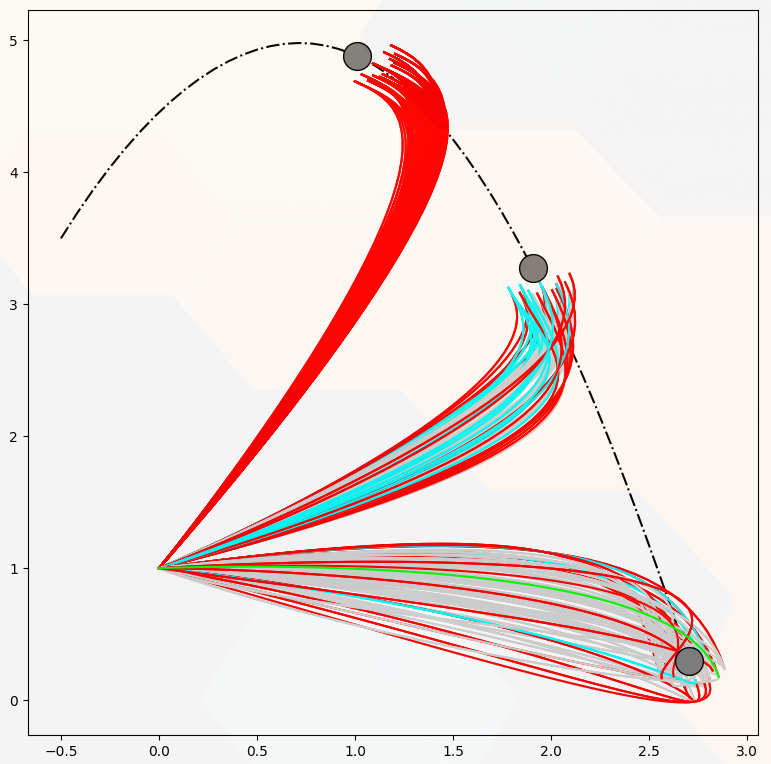
\includegraphics[width=0.7\linewidth]{generation_example.png}
	\caption{Generated trajectories for different final states and time horizons.}
\end{figure}
\section{Feasibility of Trajectories}
\label{sec:feasibility}
In the previous section, the trajectory generation approach was presented and the relation between the state trajectory and the system inputs has been established.
Still, we have to ensure the trajectory is actually feasible regarding the translational constraints in \Cref{eq:translational-constraints}, as the constraints are generally neglected during the generation stage.
The same applies to the input feasibility.
Since these constraints are not inherent to the generation stage, they can be considered as feasibility tests, classifying the given trajectory as feasible or not. 

\subsection{Input Feasibility}
\label{sec:input-feasibility}

We can split the problem of input feasibility into two subproblems, thrust feasibility and body rate feasibility. The thrust feasibility check ensures that the vehicle does not exceed its thrust capabilities denoted by $\fmin$ for the minimum and $\fmax$ for the maximum thrust it can generate.
We formulate the thrust constraints as
\begin{equation}
	\label{eq:thrust-limits}
	\unit[0]{N} \leq f_\text{min} \leq f \leq f_\text{max}
	.
\end{equation}
The body rate feasibility check declares a given state trajectory feasible if
\begin{equation}
	\label{eq:body-rates-limit}
	\left\lVert\omeb\right\rVert
	\leq
	\omega_\text{max}
\end{equation}
is guaranteed to be valid over the whole trajectory.

Both checks are applied on the trajectory per axis with sufficient but not necessary criterions for both feasibility and infeasibility. As a consequence there might be feasible (as well as infeasible) trajectories that might be classified as indeterminable. The checks are applied recursively on subsections of the whole interval $\left[0,T\right]$ in case they can not classify the section as provably feasible or unfeasible.

\subsubsection{Thrust Input Feasibility}
\begin{itemize}
	\color{red}
	\item cubic instead of quadratic function is to be solved
	\item stress out, that feasibility criterium is quite coarse -> feasible solution might be classified as indeterminable
	\item following equations are per axis. Indies are omitted if unambiguous.
\end{itemize}
We consider the interval 
\begin{equation}
	\mathcal{T} = \left[\tau_1,\tau_2\right] \subseteq \left[0,T\right]
	,
\end{equation}
for which the thrust feasibility criterion in \Cref{eq:thrust-limits} is fulfilled if and only if
\begin{align}
	\label{eq:thrust-feasibility-equivilency-max}
	\max_{t \in \mathcal{T}} f(t)^2
	&\leq
	f_\text{max}^2 \\
	\label{eq:thrust-feasibility-equivilency-min}
	\min_{t \in \mathcal{T}} f(t)^2
	&\geq
	f_\text{min}^2
	.
\end{align}

By squaring \Cref{eq:trajectory-thrust}, we can write the squared thrust in per-axis notation
\begin{equation}
	\label{eq:thrust-squared-per-axis}
	f^2 = 
	\left\lVert
	\left(m + X_{\dot{u}}\right) \pbpp + X_u \pbp
	\right\rVert^2
	= 
	\sum_{k=1}^{3}
	\left(\left(m + X_{\dot{u}}\right)\ppp_k + X_u \pp_k \right)^2
\end{equation}
and bound the thrust conservatively by summation over the per axis extrema
\begin{align}
	\label{eq:fmax-per-axis}
	\max_{t \in \mathcal{T}} f(t)^2
	&\leq
	\sum_{k=1}^{3}
	\max_{t \in \mathcal{T}}
	\left(
		\left(m + X_{\dot{u}}\right)
		\ppp_k
		+ X_u \pp_k
	\right)^2 \\
	\label{eq:fmin-per-axis}
	\min_{t \in \mathcal{T}} f(t)^2
	&\geq
	\sum_{k=1}^{3}
	\min_{t \in \mathcal{T}}
	\left(
		\left(m + X_{\dot{u}}\right)
		\ppp_k
		+ X_u \pp_k
	\right)^2
	.
\end{align}

We denote the maximum and minimum of the per axis thrust as \fmaxaxis and \fminaxis, respectively \todo{Hier ist im Unterschied zu Mueller eine kubische Funktion fuer die Nullstellen zu loesen} 
and write the extrema in \Cref{eq:fmax-per-axis,eq:fmin-per-axis} as
\begin{align}
	\max_{t \in \mathcal{T}}
	\left(
		\left(m + X_{\dot{u}}\right)
		\ppp_k
		+ X_u \pp_k
	\right)^2
	&= 
	\max\left\{\fmaxaxis^2, \fminaxis^2\right\} \\
	\min_{t \in \mathcal{T}}
	\left(
		\left(m + X_{\dot{u}}\right)
		\ppp_k
		+ X_u \pp_k
	\right)^2
	&=
	\begin{cases}
		\min\left\{\fmaxaxis^2, \fminaxis^2\right\}
		& \text{if } \fmaxaxis\cdot\fminaxis > 0 \\
		0
		& \text{otherwise}
	\end{cases}
\end{align}

A sufficient criterion, rendering the trajectory infeasible, is
\begin{equation}
	\label{eq:sufficient-infeasible-thrust}
	\max\left\{\fmaxaxis^2, \fminaxis^2\right\}
	> \fmaxsquare
	,
\end{equation}
whereas a sufficient criterion for feasibility with respect to the thrust input is if both
\begin{align}
	\label{eq:sufficient-feasible-thrust-max}
	\sum_{k=1}^{3}
	\max_{t \in \mathcal{T}}
	\left\{\fmaxaxis^2, \fminaxis^2\right\}
	& \leq
	\fmaxsquare \\
	\label{eq:sufficient-feasible-thrust-min}
	\sum_{k=1}^{3}
	\min_{t \in \mathcal{T}}
	\left\{\fmaxaxis^2, \fminaxis^2\right\}
	& \geq
	\fminsquare
\end{align}
hold. Note that it might be the case, that neither \Cref{eq:sufficient-infeasible-thrust} nor \Cref{eq:sufficient-feasible-thrust-max,eq:sufficient-feasible-thrust-min} hold. This does not necessarily mean, that the section has to be infeasible. Even though, the highest order term is $\pp_k$ of fourth order due to velocity dependent damping opposed to the \ac{uav} application in \cite{MuellerHehn15}, where it is of order three, we can still consider the per axis criteria as computationally efficient. Finding the extrema of a fourth order polynomial comes down to finding the roots of a third order polynomial, for which a closed form solution exists. Additionally, to find the extrema for the interval $\mathcal{T}$ it is sufficient to solve it once for the whole duration of the trajectory. Subsequently, we check for each interval $\mathcal{T}$, if the candidate for a local extremum lies within $\mathcal{T}$ and find the global extrema for $\mathcal{T}$ by comparing the thrusts of the respective candidate with the thrust values on the boundaries of $\mathcal{T}$. We can conclude, that in the best case, i.e. no local extremum candidate lies within $\mathcal{T}$, two function evaluations of a quartic polynomial are required. Whereas, for the worst case, i.e. all local extremum candidates lie within $\mathcal{T}$, five evaluations are required.

To obtain the thrust function in terms of the state trajectory parameters $\alpha$, $\beta$ and $\gamma$, we plug \Cref{eq:optimal-trajectory-per-axis} into \Cref{eq:trajectory-thrust}, which yields
\begin{equation}
	\begin{aligned}
		f ={}
		&\frac{X_u \alpha}{24} t^4
		+ \frac{X_u \beta + \left(m+X_{\dot{u}}\right)}{6} t^3
		+ \frac{X_u \gamma + \left(m + X_{\dot{u}}\right)}{2} t^2 \\
		& + \left(
			X_u a_0 + \left(m + X_{\dot{u}}\right) \gamma
		\right) t
		+ X_u v_0
		+ \left(m + X_{\dot{u}}\right) a_0
\end{aligned}
\end{equation}
per axis.

\begin{algorithm}
    \caption{CheckThrustFeasibility}
    \label{alg:thrust-feasibility}
	\begin{algorithmic}[1]
		\Function{CheckThrustFeasibility}{$\fmin$, $\fmax$, $\tau_1$, $\tau_2$}
		\If{$\tau_2 - \tau_1 < \tau_{\min}$}
		\Comment{Termination criterion to limit recursion depth}
			\State \textbf{return} indeterminable
		\EndIf
		% \LeftComment check the boundaries of the interval explicitly
		% \State $f_1 \gets$ \Call{Max}{\Call{Thrust}{$\tau_1$}, \Call{Thrust}{$\tau_2$}}
		% \State $f_2 \gets$ \Call{Min}{\Call{Thrust}{$\tau_1$}, \Call{Thrust}{$\tau_2$}}
		% \If{$f_1 > \fmax$}
		% 	\State \textbf{return} infeasible
		% \ElsIf{$f_2 < \fmin$}
		% 	\State \textbf{return} infeasible
		% \EndIf
		\State $\Sigma_{\min}^2 \gets 0$
		\Comment{Sum of $\min(f^2)$ over all axes}
		\State $\Sigma_{\max}^2 \gets 0$
		\Comment{Sum of $\max(f^2)$ over all axes}
		\For{all axes}
			\State $f_1, f_2 \gets \Call{MinMaxThrustOfAxis}{\tau_1, \tau_2}$
			\If{\Call{Max}{$f_1^2,f_2^2$} $> \fmax$} \Comment{a single axis exceeds $\fmax$}
				\State \textbf{return} infeasible
			\EndIf
			\If{$f_1 \cdot f_2 < 0$}
				\State $\Sigma_{\min}^2 \gets \Sigma_{\min}^2$
			\Else
				\State $\Sigma_{\min}^2 \gets \Sigma_{\min}^2 + \Call{Min}{f_1^2, f_2^2}$
			\EndIf
			\State $\Sigma_{\max}^2 \gets \Sigma_{\max}^2 + \Call{Max}{f_1^2, f_2^2}$
		\EndFor
		\If{$\Sigma_{\max}^2 < \fminsquare$}
		\Comment{Apply the infeasibility criterion}
			\State \textbf{return} infeasible
		\ElsIf{$\Sigma_{\min}^2 > \fmaxsquare$}
			\State \textbf{return} infeasible
		\EndIf
		\If{$\Sigma_{\max}^2 \leq \fmaxsquare$ and $\Sigma_{\min}^2 \geq \fminsquare$}
		\Comment{Apply the feasibility criterion}
			\State \textbf{return} feasible
		\Else \Comment{Test feasibility recursively on subintervals}
			\State $\tau_{\text{m}} \gets (\tau_1 + \tau_2) / 2$
			\If {\Call{CheckThrustFeasibility}{$\fmin,\fmax,\tau_1,\tau_{\text{m}}$} $=$ feasible}
				\State \textbf{return} \Call{CheckThrustFeasibility}{$\fmin,\fmax,\tau_{\text{m}},\tau_2$}
			\Else
				\State \textbf{return} infeasible
			\EndIf
		\EndIf
		\EndFunction
	\end{algorithmic}
\end{algorithm}

\subsubsection{Body Rates Input Feasibility}
\begin{itemize}
	\color{red}
	\item Insert dynamics into definition of jerk
\end{itemize}
We can formulate an upper bound on the body rates by applying the vector induced euclidean norm $\left\lVert\Rb\right\rVert \leq 1$ on \Cref{eq:body-rate-relation}
\begin{equation}
	\label{eq:body-rates-bound}
	\omega_3^2 + \omega_2^2 \leq
	\frac{1}{f^2}
	\left\lVert
		\left(
			m + X_{\dot{u}}
		\right) \pbppp + X_u \pbpp
	\right\rVert^2
	.
\end{equation}
A conservative upper bound of \Cref{eq:body-rates-bound} in per axis notation denoted as $\bar{\omega}^2$ can be written with \Cref{eq:thrust-squared-per-axis} as
\begin{equation}
	\omega_2^2 + \omega_3^2
	\leq
	\bar{\omega}^2
	=
	\frac{
		\sum_{k=1}^{3}
		\max_{t \in \mathcal{T}}
		\left(
			\left(
				m + X_{\dot{u}}
			\right)\dddot{p}_k + X_u \ddot{p}
		\right)^2
	}{
		\sum_{k=1}^{3}
		\min_{t \in \mathcal{T}}
		\left(
			\left(m + X_{\dot{u}}\right)\ppp_k
			+ X_u \pp_k
		\right)^2
	}
	,
\end{equation}

and simplified with \Cref{eq:sufficient-feasible-thrust-min} and defining $\xi_k = \left(m + X_{\dot{u}}\right)\dddot{p}_k + X_u \ddot{p}$ so it reads
\begin{equation}
	\bar{\omega}^2 =
	\frac{
		\sum_{k=1}^{3}
		\max_{t \in \mathcal{T}}
		\xi_k^2
	}{
		\sum_{k=1}^{3}
		\min_{t \in \mathcal{T}}
		\left\{\fmaxaxis^2, \fminaxis^2\right\}
	}
	.
\end{equation}
The minimum and maximum of $\xi_k$ is denoted as \ximaxaxis and \ximinaxis, respectively. With
\begin{equation}
	\max_{t \in \mathcal{T}}
	\left(
		\left(
			m + X_{\dot{u}}
		\right)
		\dddot{p}_k + X_u \ddot{p}
	\right)^2 =
	\max_{t \in \mathcal{T}}
	\left\{
		\ximaxaxis^2, \ximinaxis^2
	\right\}
	,
\end{equation}
we formulate the feasibility criterion with respect to the body rates
\begin{equation}
	\label{eq:body-rates-criterion-per-axis}
	\bar{\omega}^2
	=
	\frac{
		\sum_{k=1}^{3}
		\max_{t \in \mathcal{T}}
		\left\{
			\ximaxaxis^2, \ximinaxis^2
		\right\}
	}{
		\sum_{k=1}^{3}
		\min_{t \in \mathcal{T}}
		\left\{\fmaxaxis^2, \fminaxis^2\right\}
	}
	\leq
	\omegamaxsquare
	.
\end{equation}
This body rate feasibility criterion is analogous to the upper bound criterion for the thrust feasibility in \Cref{eq:sufficient-feasible-thrust-max}. If \Cref{eq:body-rates-criterion-per-axis} does not hold, the tested interval $\mathcal{T}$ is split in half and the feasibility criterion is applied recursively on both subintervals, subsequently.


\subsection{Translational Constraints Feasibility}
At this stage we can check if a trajectory meets the requirements for being classified as input feasible as presented in \Cref{sec:input-feasibility}. Still there is no guarantee, the trajectory will not violate the translational constraints formulated in \Cref{eq:translational-constraints}.

\subsubsection{Position Feasibility}
\label{sec:position-feasibility}
We can formulate position constraints as planes. We define the allowable side of the plane by a normal vector $\nb_{\text{p}}$. We call this kind of positional constraints wall constraints. These wall constraints can be used to encode the constraints due to local conditions, such as the water surface or the walls of a confined environment, the vehicle is not allowed or able to cross. Feasibility has to be tested for critical points only. The critical points are those meeting the sufficient criterion for being at a minimal distance to the plane encoding the wall constraint. We find the critical points by finding the roots of $\pp_{\text{n}}(t) = \nb_{\text{p}}^\top \, \pbp(t)$.
\begin{equation}
	\mathcal{C}_{\text{crit}} =
	\left\{
		t \in \left[ 0, T \right]
		\,\mid\, \pp_{\text{n}}(t) = 0
	\right\}
	\cup
	\left\{0,T\right\}
\end{equation}

The trajectory is feasible with respect to the position constraints if and only if
\begin{equation}
	\label{eq:position-feasibility-criterion}
	\nb_\text{p}^\top
	\left(
		\pbo(t) - \pbo_{\text{p}}
	\right)
	> 0
	\,\forall\, t \in \mathcal{C}_{\text{crit}}
	,
\end{equation}
with $\pbo_{\text{W}}$ denoting an arbitrary point on the plane defining the wall constraint. Geometrically interpreted, we can regard $\pp_{\text{n}}$ as the velocity projected onto the normal direction of the plane given by $\nb_{\text{W}}$.

The position is a quintic polynomial, as we can see in \Cref{eq:optimal-trajectory-per-axis}. Thus, computing $\mathcal{C}_{\text{crit}}$ is done by solving the roots of the fourth order polynomial $\pp_{\text{n}}$. The feasibility check is carried out by evaluating the left-hand side of \Cref{eq:position-feasibility-criterion} at least twice and most six times per axis. This is similar to the input feasibility checks presented in \Cref{sec:input-feasibility} with the difference that no recursion is needed, though.

\subsubsection{Velocity Feasibility}

\todo{optional}

\section{Obstacle/Collision Avoidance}

\begin{itemize}
	\color{red}
	\item Make clear, that obstacle avoidance is not built into the trajectory generation itself. 
	\item can be seen as subsequent feasibility check. 
\end{itemize}

\todo[inline]{Reference \cite{Bucki19}}
As for the translational constraints and the input feasibility, collision avoidance is not inherent to the generation of trajectories, but is applied as a test afterwards. Trajectories failing the test are discarded.
Obstacle avoidance can be added to the trajectory planning straightforwardly by extending the position feasibility test in \Cref{sec:position-feasibility}.
Instead of checking for a collision with a single predefined plane, the position check is performed recursively on subintervals of $\left[0, T\right]$.
For each recursion, a plane separating the section of the trajectory from the convex obstacle $\mathcal{O}$ is defined.
The position feasibility check is performed and if the whole section lies on the allowable side of separating plane, i.e. in the direction away from the object, the section is declared feasible.
Otherwise, the check is performed recursively on the subinterval including the intersection with the separating plane.
The interested reader may refer to \cite{Bucki19} for an exhaustive analysis of such a collision avoidance algorithm in the domain of aerial vehicles.
The pseudocode describing an algorithm performing the collision feasibility test can be seen in \Cref{alg:collision-detection}.
\begin{algorithm}
    \caption{Collision Detection based on \cite{Bucki19}}
    \label{alg:collision-detection}
	\begin{algorithmic}[1]
		\Require $\pbo(0),\pbo(T) \notin \mathcal{O}$
		\Function{CollisionFeasibility}($\tau_{\min}$)
			\If{not $\pbo(0),\pbo(T) \notin \mathcal{O}$}
				\State \textbf{return} infeasible
			\EndIf
			\State \textbf{return}
			\Call{CollisionCheck}{$0, T$}
		\EndFunction
		\Function{CollisionCheck}{$\tau_1, \tau_2$}
		\State $\tau_{\text{mid}} \gets (\tau_1 + \tau_2) / 2$
		\If{$\pbo(\tau_{\text{mid}}) \in \mathcal{O}$}
			\State \textbf{return} infeasible
		\ElsIf{$\tau_2 - \tau_1 < \tau_{\min}$}
			\State \textbf{return} indeterminable
		\EndIf
		\State $\pbo_{\text{p}}, \nb_{\text{p}} \gets$
		\Call{GetSeparatingPlane}{$\pbo(\tau_{\text{mid}}),\mathcal{O}$}
		\State $\mathcal{C}_{\text{crit}} \gets
		\left\{
			t \in \left[ \tau_{\text{mid}}, \tau_2 \right]
			\,\mid\, \pp_{\text{n}}(t) = 0
		\right\}$ in ascending order
		\For{$t_i$ in $\mathcal{C}_{\text{crit}}$, skipping $\tau_{\text{mid}}$}
			\If{$\nb_\text{p}^\top
				\left(
					\pbo(t_i) - \pbo_{\text{p}}
				\right)
				\leq 0$}
				\State result $\gets$ \Call{CollisionCheck}{$t_{i-1},\tau_2$}
				\If{result = feasible}
					\State \textbf{break}
				\Else
					\State \textbf{return} result
					\Comment{either infeasible or indeterminable}
				\EndIf
			\EndIf
		\EndFor
		\State $\mathcal{C}_{\text{crit}} \gets
		\left\{
			t \in \left[ \tau_1, \tau_{\text{mid}}\right]
			\,\mid\, \pp_{\text{n}}(t) = 0
		\right\}$ in descending order
		\For{$t_i$ in $\mathcal{C}_{\text{crit}}$, skipping $\tau_{\text{mid}}$}
			\If{$\nb_\text{p}^\top
			\left(
				\pbo(t_i) - \pbo_{\text{p}}
			\right)
			\leq 0$}
				\State \textbf{return} \Call{CollisionCheck}{$\tau_1, \tau_{\text{mid}}$}
			\EndIf
		\EndFor
		\State \textbf{return} feasible
		\EndFunction
	\end{algorithmic}
\end{algorithm}

The recursion depth of \Cref{alg:collision-detection} is limited by $\tau_{\min}$.
If an examined section of the trajectory bounded by the time interval $\left[\tau_1, \tau_2\right]$ becomes small enough that $\tau_2 - \tau_1 < \tau_{\min}$, the trajectory is declared indeterminable.
Computation time wise, we can expect the choice of $\tau_{\min}$ to have a significant influence for indeterminable trajectories.
This is, because $\tau_{\min}$ limits the recursion depth in case no subinterval has been declared infeasible yet, nor could feasibility be guaranteed for the whole interval $\left[0, T\right]$.
Choosing $\tau_{\min}$ larger reduces the time required in case feasibility could not be decided upon before splitting the interval in smaller sections than $\tau_{\min}$.
On the other hand, choosing $\tau_{\min}$ smaller could result in trajectories being declared as feasible, that would have been discarded as indeterminable otherwise.

Note that we are not restricted to static obstacles by this approach of obstacle avoidance. We define the trajectory of the relative position of the vehicle to the obstacle as
\begin{equation}
	\pbs(t) = \pbo(t) - \pbo_{\mathcal{O}}(t)
	,
\end{equation}
where $\pbo_{\mathcal{O}}(t)$ denotes the obstacle's trajectory. Instead of performing the collision check for $\pbo$, we do it for $\pbs$. In general, $\pbo_{\mathcal{O}}$ and consequently $\pbs$ could be arbitrary functions of time.
But choosing them not to be a polynomial of order at most five, would render the collision avoidance significantly less computational efficient. Hence, we assume the trajectories being of at most order five, and the collision avoidance being performable by solving roots of quartic polynomials.

\begin{tikzpicture}
    \begin{axis}[
            xmin=-2,xmax=1,
            ymin=-3,ymax=3,
            grid=both,
            ]
            \addplot [domain=-0.5:3.5,samples=50]({-1.083 * x^3 + 5.25 * x^2 -6.67*x + 1},{0.167 * x^3 - 0.25 * x^2 + 0.583 *x - 2}); 
    \end{axis}
\end{tikzpicture}

\section{Control}
\label{sec:control}
\begin{itemize}
	\color{red}
	\item one could use the min jerk trajectory approach simply for generation -> feed-back control to keep the vehicle on track
	\item computational efficiency and real-time capability of approach enables trajectory generation to be used for implicit feedback. Regenerate trajectories in each control time step.
	\item body rates will change rather slowly compared to quadrocopters -> instead of using body rates as in MuellerHehn15, use target attitude and attitude control (actually the body rates are derived from a target attitude anyway)
\end{itemize}
While we attended to the generation and planning of trajectories and the question of feasibility regarding vehicle dynamics, translational constraints and collision avoidance in the previous sections, this section is about tracking the obtained trajectories.

The general control architecture implements the inner-outer loop control scheme as depicted in \Cref{fig:inner-outer-loop-feedback-control}.
\begin{figure}
	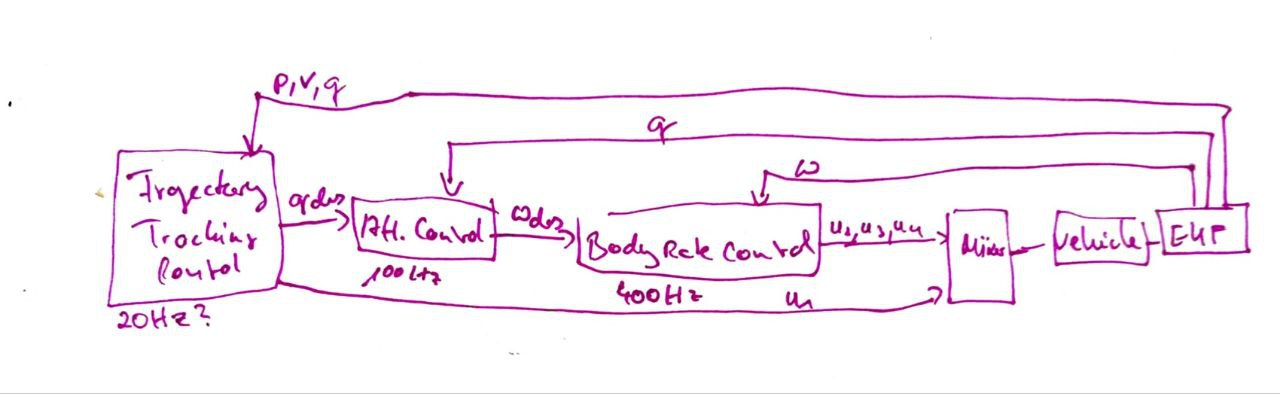
\includegraphics[width=0.8\textwidth]{inner-outer-loop}
	\caption{Overview of the control loops.}
	\label{fig:inner-outer-loop-feedback-control}
\end{figure}
The authors in \cite{Maurya09} demonstrated the viability of this approach for marine vehicles. The basic idea is to divide the problem of trajectory into easier to solve sub problems. By inner loops we refer to the low-level dynamic control loops consisting of attitude or body rate controllers. The design and tuning of these inner loops are highly dependent on the vehicle dynamics. The outer control loops, for example a position, path, or trajectory tracking controller, can be considered as kinematic control loops. They are by design decoupled from vehicle dynamics under the assumption, that the inner control loops are fast enough to reach the target value instantaneously from the perspective of the outer loop. This is equivalent to the assumption in \Cref{sec:thruster-model}, that the thruster dynamics compared to the \ac{uauv} dynamics are sufficiently fast to be negligible. As a result, we have a fast-slow separation from inner to outer loop, i.e. the inner loops run with a significantly higher frequency than the outer ones.

\subsection{Body Rate Control}
The body rate controller represents the innermost control loop.

We define the error of the angular velocity and acceleration in the body-fixed frame $\mathcal{B}$
\begin{equation}
	\vangerror = \vangbody - \vangdesiredbody \quad \text{and }
	\aangerror = \aangbody - \aangdesiredbody
	,
\end{equation}
and the control law for controlling $\vangbody$, reading
\begin{equation}
	\begin{bmatrix}
		u_2 \\ u_3 \\ u_4
	\end{bmatrix}
	=
	\KpBodyRate \vangerror
	+ \KiBodyRate \int_{}^{t} \vangerror(\tau)\text{d}\tau
	+ \KdBodyRate \aangerror
	+\underbrace{
		\vangdesiredbody \times \Jbs \vangdesiredbody
		+ \Domegaadded \vangdesiredbody
		- \vlinbody \times \Mbs \vangdesiredbody
	}_{\text{feed forward}}
	,
\end{equation}
\todo{add p and d term and we have pid with feedfoward. }
where the feed forward terms are based on vehicle dynamics in \Cref{eq:eom-rotational-with-input}. The control law displays a PID-Controller with feed forward term, where $\KpBodyRate$, $\KiBodyRate$ and $\KdBodyRate$ are diagonal matrices denoting the proportional, integral and derivative gain, respectively.

We set $\aangdesiredbody = \unit[0]{rad/s^2}$ and observe that the input for the body rate controller is $\vangdesiredbody$. We will see in \Cref{sec:implicit-feedback-control} the usefulness of this for the implicit feedback control scheme in the context of the trajectory generation system, given the inner-outer loop assumptions hold.

\subsection{Attitude Control}
The attitude controller is the next controller upstream of the body rate controller. Hence, we consider it to be a kinematic controller with a desired body rate $\vangdesiredbody$ as output, instead of the vehicle's system inputs $\inputbody$. We define the desired thrust axis as the controller's input 
\begin{equation}
	\exdesiredbodyinworld =
	\frac{\thrustdesiredworld}{
		\left\lVert\thrustdesiredworld\right\rVert
	}
\end{equation}
and the current thrust axis, that is equivalent to 
\begin{equation}
	\exbodyinworld = \qactual \odot \eb_1
\end{equation},
where $\qactual \odot \eb_1$ denotes the rotation of the vector $\eb_1$ by the quaternion $\qactual$ and $\qactual$ is the current attitude of the vehicle.

The euler parameter representation of the rotation aligning $\exbodyinworld$ and $\exdesiredbodyinworld$ is given by
\begin{equation}
	\kb = \frac{
		\exbodyinworld \times \exdesiredbodyinworld
	}{
		\left\lVert
			\exbodyinworld \times \exdesiredbodyinworld
		\right\rVert
	}
	\quad \text{and} \quad
	\alpha = \arccos\left(\exbodyinworld \exdesiredbodyinworld\right)
\end{equation}

\subsection{Implicit Feedback Control}
\label{sec:implicit-feedback-control}

\begin{figure}[h!]
	\centering
	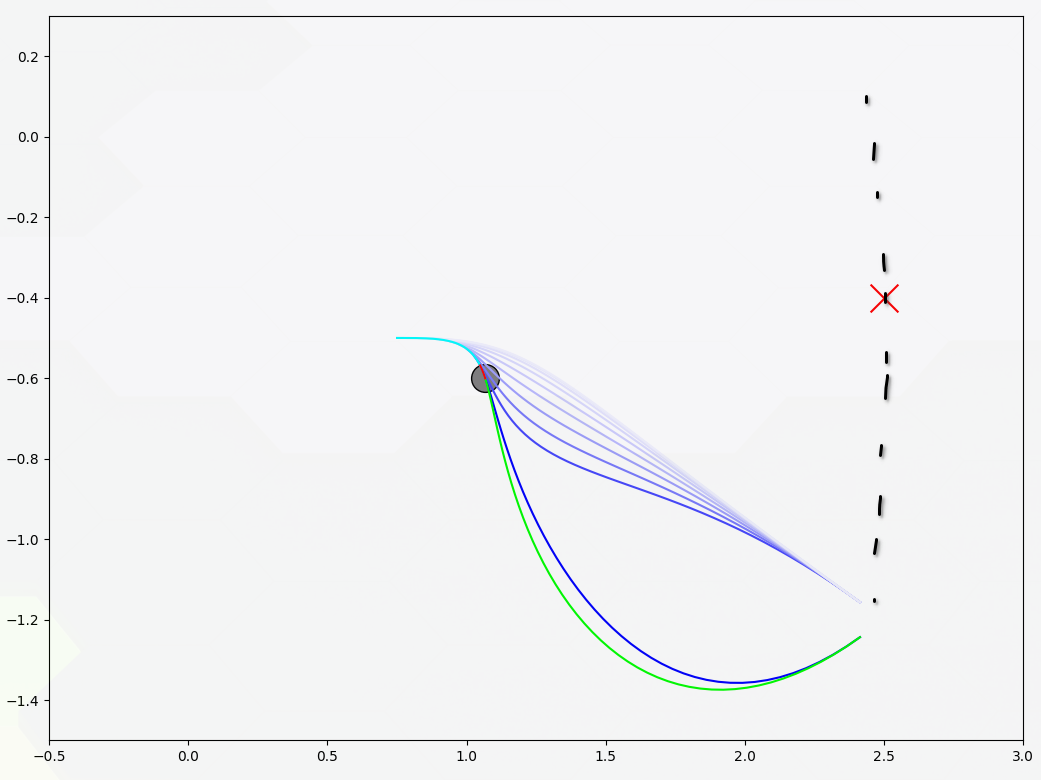
\includegraphics[width=0.8\textwidth]{trajectory-replanning}
	\caption{Implicit feedback control by regenerating new trajectories and selecting the best in each step.}
\end{figure}

One advantage of the presented trajectory generation approach is, that it is computationally cheap. Hence, we can use the trajectory generation for implicit feedback control, due to the real-time capability of the trajectory planning. We are able to resample thousands of trajectories per control update step and choose the one best suited to accomplish a certain high level task.
Subsequently, we need to recover the required thrust vector and commands for the rotational dynamics of the vehicle.

First, we compute the thrust vector $\thrustdesiredworld$ of the current trajectory at $t+\Delta T_\text{s}$, where $\Delta T_{\text{s}}$ is the update interval for the trajectory sampling, by applying the relation in \Cref{eq:trajectory-acceleration-eom} on the current trajectory.
We compute the axis of rotation $\kb$ and the corresponding angle of rotation $\alpha$ required for aligning the current forward axis of the vehicle $\exbodyinworld$ with $\thrustdesiredworld$ by
\begin{equation}
	\label{eq:rotation-to-desired-thrust-vector}
	\kb = \frac{
		\exbodyinworld \times \thrustdesiredworld
	}{
		\left\lVert
			\exbodyinworld \times \thrustdesiredworld
		\right\rVert}
	\quad
	\text{and}
	\quad
	\alpha = \arccos\left(
		\exbodyinworld \cdot
		\frac{\thrustdesiredworld}{\left\lVert\thrustdesiredworld\right\rVert}
	\right)
	.
\end{equation}
In general, it is also possible to rotate $\exbodyinworld$ by $-\alpha$ around $-\kb$ to align it with $\thrustdesiredworld$. Hence, we invert the signs of $\alpha$ and $\kb$ in case $\lvert\alpha\rvert > \pi$, so we always get the shortest rotation. \todo{not necessary, since we multiply $\alpha$ and $\kb$?}

From \Cref{eq:rotation-to-desired-thrust-vector} we compute the body rates required to align $\exbodyinworld$ with $\thrustdesiredworld$ in time $\Delta T_{\text{s}}$ directly
\begin{equation}
	\vangdesiredworld = \frac{\alpha}{\Delta T_{\text{s}}} \kb
\end{equation}

We close the feedback loop for the trajectory tracking implicitly, i.e. we compute $\thrustdesiredworld$ and $\vangdesiredworld$ in each control loop for a newly generated trajectory.
Therefore, disturbances and model inaccuracies can be compensated, because the new initial state of the generated trajectories is the actual state of the \ac{uauv}.

\subsection{Trajectory Tracking Feedback Control}
\begin{itemize}
	\item \cite{Maurya09} suggests inner-outer-loop. slow-fast, dynamic-kinematic. -> i want to go with this.
\end{itemize}
There might be cases, for those it is desirable or even necessary to track a given trajectory for a longer period then $\Delta T_{\text{s}}$ before being given a new trajectory to track.
For example, when all newly generated trajectories become infeasible. According to \cite{MuellerHehn15} this is to be expected, when the duration of the sampled trajectories becomes small.
As a consequence input feasibility checks will fail and render all trajectories infeasible.
But even for sufficiently large durations, the feasibility still depends on the combination of the initial state and the desired final state.
While we can try to choose appropriate final states, to increase the probability of getting feasible trajectories, there is no way we can influence the initial state, as it is the actual state of the \ac{uauv}.
In this case, there is no trajectory available and the implicit feedback control from the previous section can not be applied.

Theoretically, we could simply compute $\thrustdesiredworld$ and $\vangdesiredworld$ over the remainder of the last planned feasible trajectory.
In practice, model inaccuracies and external disturbances will cause the actual trajectory to diverge from the planned desired trajectory over time.
We tackle this issue by extending the architecture by a trajectory tracking feedback controller.

For the trajectory tracking, we will design a control law based on the one proposed in \cite{MellingerKumar11} for a quadrocopter tracking minimum snap trajectories.

Given a desired trajectory $\bm{\sigma}_{\text{des}}(t) = \left[\pbo(t), \phi(t)\right]^\top$, we define the position and velocity error as
\begin{equation}
	\eb_{p} = \pbo - \pbo_{\text{des}}
\end{equation}
and
\begin{equation}
	\eb_{v} = \pbp - \pbp_{\text{des}}
	,
\end{equation}
respectively.

Considering the translational dynamics of the \ac{uauv} in \Cref{eq:eom-translational-with-input}, we formulate the control law
\begin{equation}
	\label{eq:translational-control-law-short}
	u_1 = \exbodyinworld^\top \thrustdesiredworld
\end{equation}
with
\begin{equation}
	\thrustdesiredworld =
	-\Kb_p \eb_p
	- \Kb_v \eb_v
	+ \hat{\bm{M}} \pbpp
	+ \hat{\bm{D}} \pbp
	,
\end{equation}
where $\Kb_p$ and $\Kb_v$ denote diagonal gain matrices and $\hat{\bm{M}} \pbpp$ and $\hat{\bm{D}}\pbp$ represent feed forward terms. Note that $u_1$ is scaled by the projection of $\thrustdesiredworld$ onto the current body axis $\exbodyinworld$.

The advantages of this are two-fold. First, the closer $\thrustdesiredworld$ and $\exbodyinworld$ get of becoming perpendicular, the smaller $u_1$ will become. Therefore, more of the available thruster output can be allocated to minimize the attitude error. Second, for $\thrustdesiredworld$ and $\exbodyinworld$ we can see that $u_1$ can become negative. While usually not useful in the typical application of \acp{uav}, where the thrusters' direction of rotation is not reversible, \acp{uauv} can make use of backward directed thrust to minimize the translational errors $\eb_p$ and $\eb_v$. In case this should not be desired, though, we can still set $u_1=0$ if $\exbodyinworld^\top \thrustdesiredworld < 0$. Accordingly, we reformulate \Cref{eq:translational-control-law-short}
\begin{equation}
	u_1 = 
	\begin{cases}
		\exbodyinworld^T \thrustdesiredworld & \text{if } \exbodyinworld^T \thrustdesiredworld > 0 \\
		0 & \text{else.}
	\end{cases}
	!
\end{equation}




\section{Implementation}
\begin{figure}
	\centering
	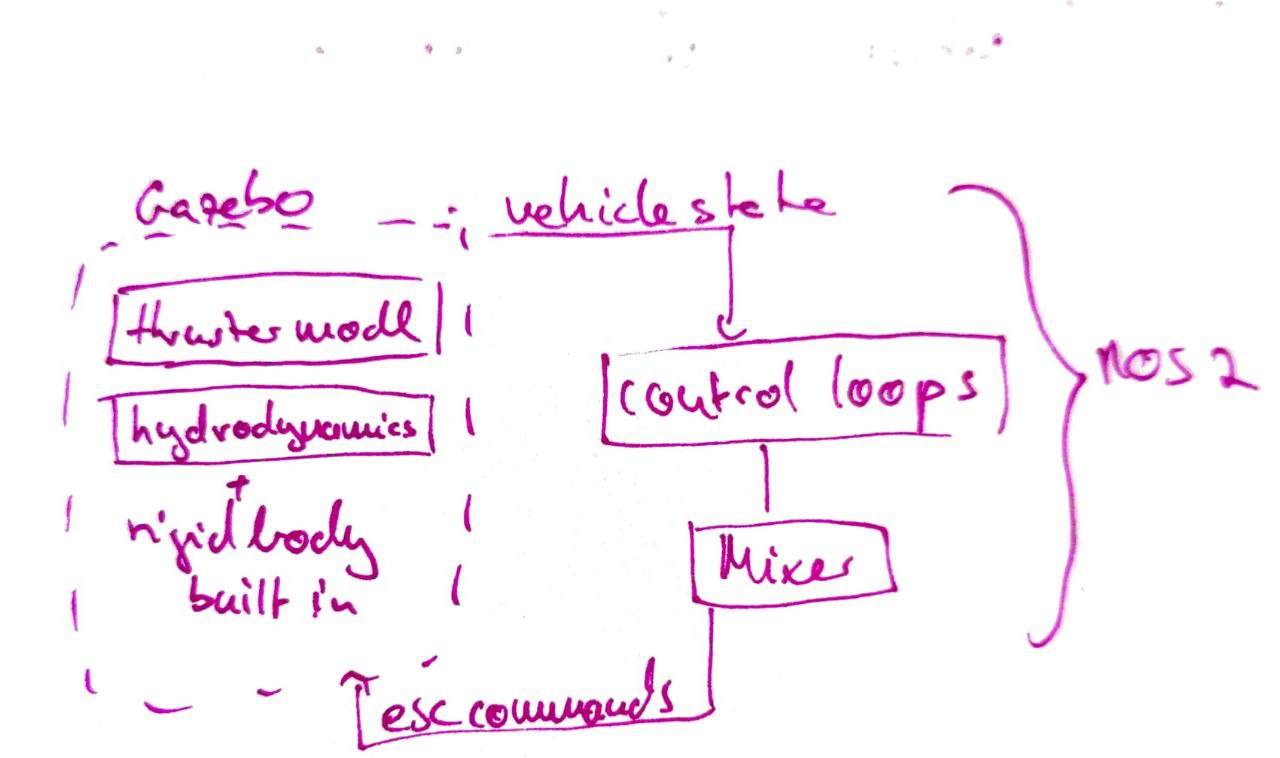
\includegraphics[width=0.5\textwidth]{gazebo-ros-interaction}
\end{figure}
\label{sec:implementation}

% !TeX root = ../Thesis.tex
\chapter{Analysis}
\begin{itemize}
	\color{red}
	\item Test the dynamic behavior of the body rates to assess whether the assumptions that they are reached slowly and by far not instantaneously holds.
	\item real time capability on limited hardware is required for deployment -> analysis of computation times required for assessment
	\item single trajectory tracking without implicit feedback, to analyze performance of (half) open loop trajectory tracking. while keeping disturbances at a minimum, this should show how susceptible the tracking performance is for errors in the assumed model parameters.
	\item Multi Trajectory/Implicit Feedback should show the full capability of the approach. Collision avoidance can be added optionally
\end{itemize}

\textcolor{blue}{
\section{(Experimental) Setup}
\begin{itemize}
    \item size of tank etc fresh water  / apriltag array inside
    \item add figure
\end{itemize}
\begin{table}[]
        \caption{Overview on ....}
		%\hspace*{-1.5cm}  % move table down (left in landscape) - tabular width: 
		\centering
		% change column width: >{\hsize=1.5\hsize\linewidth=\hsize}
		% >{\hsize=0.5\hsize\linewidth=\hsize}
		\begin{NiceTabular}
            {
            %%%%% Leider scheint die beste Methode wirklich hardgecodete Spaltenbreiten zu sein - hier am Ende rumspielen
            >{\centering\arraybackslash}m{3cm}  %
            >{\centering\arraybackslash}m{3cm} % 
            }
            \toprule
            %%%%%%%%%%% Top row - names of each columns
            Parameter &  Value \\  
            \midrule 
            %%%%%%%% Beispiel
            mass $m$ & $1$\,kg \\
            \bottomrule
		\end{NiceTabular}
		\label{tab:parameters}
\end{table}
\subsection{Qualisys Motion Capture System}
\begin{itemize}
    \item Figure sketch - 4 cameras inside the tank (+ maybe screenshot from QTM?)
    \item photo of sexy blue glowing cameras
    \item photo of hippocampus with reflective markers
    \item after conducting the QTM calibration procedure the estimated accuracy wihtin the calibration is XXXXXX according to the QTM calibration process.
\end{itemize}
}


\section{Body Rates Analysis}

\begin{itemize}
	\color{red}
	\item Useful for myself to get reasonable values for the body rate limit
	\item Either use the body rate controller or just feed through
	\item Use step function and compute the time constant?
	\item Only test pitch/yaw. Roll is irrelevant
\end{itemize}

\section{Computational Performance}

\begin{itemize}
	\color{red}
	\item Measure the following
	\begin{itemize}
		\item generation time (expected to be constant, small variance due to running on a best effort machine)
		\item input feasibility (a recursive algorithm. maybe have a special look on worst case)
		\item position feasibility (only extrema need to be considered. small variance expected)
		\item collision avoidance ()
	\end{itemize}
	\item Tabular, or BoxPlot? Or Barplot? 
\end{itemize}

\section{Single Trajectory Tracking}


\section{Implicit Feedback}
% !TeX root = ../Thesis.tex
\chapter{Conclusion}\label{chap:conclusion}
\section{Summary}
\section{Future Work}
\begin{itemize}
    \item Use thrust input from trajectory as feed forward in combination with velocity/acceleration controller.
    \item Extend obstacle avoidance to work with moving obstacles
    \item Can the approach be extended to allow for negative thrust?
\end{itemize}


% Literaturverzeichnis ins Inhaltsverzeichnis integrieren
\ifthenelse{\equal{\Sprache}{0}}
	{\bibliographystyle{mum_deu} % deutsches Lit.verzeichnis
	}{}
\ifthenelse{\equal{\Sprache}{1}}
	{\bibliographystyle{mum_en} % englisches Lit.verzeichnis z.B. statt "S." nun "p." bzw. "pp."
	}{}
	
\phantomsection %-> damit hyperref den Link richtig auf die erste Seite vom Literaturverzeichnis legt

\ifthenelse{\equal{\Sprache}{0}}
	{\addcontentsline{toc}{chapter}{Literaturverzeichnis}
	}{}
\ifthenelse{\equal{\Sprache}{1}}
	{\addcontentsline{toc}{chapter}{Bibliography}
	}{}
%\addcontentsline{toc}{chapter}{Literaturverzeichnis}
\bibliography{Literatur}



% Erklärung
\thispagestyle{empty}\cleardoublepage
%Selbstständigkeitserklärung

\thispagestyle{plain}
\large
\selectlanguage{ngerman}
%\begin{flushright}
%  Hamburg, den \today
%\end{flushright}
\textbf{Erklärung}
\vspace*{5mm}

Ich, {\VornameDesStudenten \ \NachnameDesStudenten} (\Studiengang~an der Technischen 
Universität Hamburg, Matrikelnummer \Matrikelnummer), versichere, dass ich die vorliegende 
\RemoveSpaces{		
		{\ifthenelse{\equal{\MScBSc}{0}}
			{Bachelorarbeit}{}
		\ifthenelse{\equal{\MScBSc}{1}}
			{Projektarbeit}{}
		\ifthenelse{\equal{\MScBSc}{2}}
			{Masterarbeit}{}}}
selbstständig verfasst und keine anderen als die angegebenen Hilfsmittel verwendet habe. Die Arbeit wurde in dieser oder ähnlicher Form noch keiner Prüfungskommission vorgelegt.\\

\vspace*{50mm}

\begin{center}
\noindent\begin{tabular}{c}
\makebox[\widthof{\VornameDesStudenten\NachnameDesStudenten}+1in]{\hrulefill}\\
{ Unterschrift} \\[8ex]% adds space between the two sets of signatures
\end{tabular}
\noindent\begin{tabular}{c}
\makebox[1.75in]{\hrulefill}\\
Datum\\[8ex]
\end{tabular}
\end{center}
  


\normalsize

\end{document}

%##########################################################################
